% !TeX encoding = UTF-8
% !TeX program = xelatex
% !TeX spellcheck = en_US

\documentclass[degree=bachelor,fontset=windows]{thuthesis}
  % 学位 degree:
  %   doctor | master | bachelor | postdoc
  % 学位类型 degree-type:
  %   academic(默认)| professional
  % 语言 language
  %   chinese(默认)| english
  % 字体库 fontset
  %   windows | mac | fandol | ubuntu
  % 建议终版使用 Windows 平台的字体编译


% 论文基本配置,加载宏包等全局配置
% !TeX root = ./thuthesis-example.tex

% 论文基本信息配置

\thusetup{
  %******************************
  % 注意:
  %   1. 配置里面不要出现空行
  %   2. 不需要的配置信息可以删除
  %   3. 建议先阅读文档中所有关于选项的说明
  %******************************
  %
  % 输出格式
  %   选择打印版(print)或用于提交的电子版(electronic),前者会插入空白页以便直接双面打印
  %
  output = electronic,
  % 格式类型
  %   默认为论文(thesis),也可以设置为开题报告(proposal)
  % thesis-type = proposal,
  %
  % 标题
  %   可使用“\\”命令手动控制换行
  %
  title  = {水密流形三维网格重建与逆渲染},
  title* = {Watertight manifold mesh reconstruction and inverse rendering},
  %
  % 学科门类
  %   1. 学术型
  %      - 中文
  %        需注明所属的学科门类,例如:
  %        哲学、经济学、法学、教育学、文学、历史学、理学、工学、农学、医学、
  %        军事学、管理学、艺术学
  %      - 英文
  %        博士:Doctor of Philosophy
  %        硕士:
  %          哲学、文学、历史学、法学、教育学、艺术学门类,公共管理学科
  %          填写“Master of Arts“,其它填写“Master of Science”
  %   2. 专业型
  %      直接填写专业学位的名称,例如:
  %      教育博士、工程硕士等
  %      Doctor of Education, Master of Engineering
  %   3. 本科生不需要填写
  %
  degree-category  = {工学学士},
  degree-category* = {Bachelor of Science},
  %
  % 培养单位
  %   填写所属院系的全名
  %
  department = {交叉信息研究院},
  %
  % 学科
  %   1. 研究生学术型学位,获得一级学科授权的学科填写一级学科名称,其他填写二级学科名称
  %   2. 本科生填写专业名称,第二学位论文需标注“(第二学位)”
  %
  discipline  = {计算机科学与技术},
  discipline* = {Computer Science and Technology},
  %
  % 专业领域
  %   1. 设置专业领域的专业学位类别,填写相应专业领域名称
  %   2. 2019 级及之前工程硕士学位论文,在 `engineering-field` 填写相应工程领域名称
  %   3. 其他专业学位类别的学位论文无需此信息
  %
  % professional-field  = {计算机技术},
  % professional-field* = {Computer Technology},
  %
  % 姓名
  %
  author  = {李宗泰},
  author* = {Zongtai Li},
  %
  % 指导教师
  %   中文姓名和职称之间以英文逗号“,”分开,下同
  %
  supervisor  = {杜韬, 助理教授},
  supervisor* = {Professor Tao Du},
  %
  % 副指导教师
  %
  % associate-supervisor  = {陈文光, 教授},
  % associate-supervisor* = {Professor Chen Wenguang},
  %
  % 联合指导教师
  %
  % co-supervisor  = {某某某, 教授},
  % co-supervisor* = {Professor Mou Moumou},
  %
  % 日期
  %   使用 ISO 格式;默认为当前时间
  %
  % date = {2019-07-07},
  %
  % 是否在中文封面后的空白页生成书脊(默认 false)
  %
  include-spine = false,
  %
  % 密级和年限
  %   秘密, 机密, 绝密
  %
  % secret-level = {秘密},
  % secret-year  = {10},
  %
  % 博士后专有部分
  %
  % clc                = {分类号},
  % udc                = {UDC},
  % id                 = {编号},
  % discipline-level-1 = {计算机科学与技术},  % 流动站(一级学科)名称
  % discipline-level-2 = {系统结构},          % 专业(二级学科)名称
  % start-date         = {2011-07-01},        % 研究工作起始时间
}

% 载入所需的宏包

% 定理类环境宏包
\usepackage{amsthm}
% 也可以使用 ntheorem
% \usepackage[amsmath,thmmarks,hyperref]{ntheorem}

\thusetup{
  %
  % 数学字体
  % math-style = GB,  % GB | ISO | TeX
  math-font  = xits,  % stix | xits | libertinus
}

% 可以使用 nomencl 生成符号和缩略语说明
% \usepackage{nomencl}
% \makenomenclature

% 表格加脚注
\usepackage{threeparttable}

% 表格中支持跨行
\usepackage{multirow}

% 固定宽度的表格。
% \usepackage{tabularx}

% 跨页表格
\usepackage{longtable}

% 算法
\usepackage{algorithm}
\usepackage{algorithmic}

% 量和单位
\usepackage{siunitx}

% 参考文献使用 BibTeX + natbib 宏包
% 顺序编码制
\usepackage[sort]{natbib}
\bibliographystyle{thuthesis-numeric}

% 著者-出版年制
% \usepackage{natbib}
% \bibliographystyle{thuthesis-author-year}

% 生命科学学院要求使用 Cell 参考文献格式(2023 年以前使用 author-date 格式)
% \usepackage{natbib}
% \bibliographystyle{cell}

% 本科生参考文献的著录格式
% \usepackage[sort]{natbib}
% \bibliographystyle{thuthesis-bachelor}

% 参考文献使用 BibLaTeX 宏包
% \usepackage[style=thuthesis-numeric]{biblatex}
% \usepackage[style=thuthesis-author-year]{biblatex}
% \usepackage[style=gb7714-2015]{biblatex}
% \usepackage[style=apa]{biblatex}
% \usepackage[style=mla-new]{biblatex}
% 声明 BibLaTeX 的数据库
% \addbibresource{ref/refs.bib}

% 定义所有的图片文件在 figures 子目录下
\graphicspath{{figures/}}

% 数学命令
\makeatletter
\newcommand\dif{%  % 微分符号
  \mathop{}\!%
  \ifthu@math@style@TeX
    d%
  \else
    \mathrm{d}%
  \fi
}
\makeatother

% hyperref 宏包在最后调用
\usepackage{hyperref}



\begin{document}

% 封面
\maketitle

% 学位论文指导小组、公开评阅人和答辩委员会名单
% 本科生不需要
% \input{data/committee}

% 使用授权的说明
% 本科生开题报告不需要
% \copyrightpage
% 将签字扫描后授权文件 scan-copyright.pdf 替换原始页面
% \copyrightpage[file=scan-copyright.pdf]

\frontmatter
% !TeX root = ../thuthesis-example.tex

% 中英文摘要和关键字

\begin{abstract}
  三维重建与逆渲染,即从多视角图像中重建物体的三维几何结构、表面材质和环境照明,是计算机视觉和计算机图形学领域中非常重要的一个问题。在本文中,我们提出了一种新的方法来解决三维重建和逆渲染问题。值得一提的是,我们的方法考虑了间接光照和遮挡,并较为精确地重建了物体的漫反射颜色,而现有方法还原的漫反射颜色通常会受到阴影和间接光照的影响。我们的方法的关键在于一种交替优化的框架,交替优化可微光栅化和可微光线追踪。首先,我们借助 修改版 TensoIR 来初始化密度和 BRDF 参数的空间场。接下来,我们的方法在两个优化过程之间交替进行。首先,我们使用可微光栅化来进一步优化密度场和参数场。我们通过可微 Marching Cube 提取物体的几何表面信息,并使用标准光栅化进行第一次渲染。然后,我们固定重建的几何信息,通过可微光线追踪框架优化材质和照明参数。在之后的反复训练中,我们将可微光线追踪优化的间接光照进一步结合到可微光栅化中,以鼓励生成更准确的材质信息。我们的框架在可微光栅化中优化几何,在可微光线追踪中模拟准确的全局照明和光线传输,最终产生比单独使用可微分光栅化或光线追踪更准确的几何、材质和环境光照。
  % 关键词用“英文逗号”分隔,输出时会自动处理为正确的分隔符
  \thusetup{
    keywords = {三维重建,逆渲染,可微光栅化,可微光线追踪},
  }
\end{abstract}

\begin{abstract*}
  Inverse rendering is a crucial problem in computer graphics and computer vision, aiming to reconstruct the three-dimensional geometry, surface materials, and environmental illumination of objects from multi-view images. In this paper, we present a novel method to address the inverse rendering problem. Notably, our method takes indirect light and occlusion into consideration and recovers albedo maps of objects free of baked illumination artifacts, which are common in baseline methods. The key of our method is an alternating optimization framework involving both differentiable rasterization and differentiable ray tracing. First, we pre-train TensoIR to initialize spatial fields of densities and BRDF parameters. Next, our method alternates between 2 optimization procedures. First, we use differentiable rasterizer to further optimize the density field, parameter field, by extracting the surface with differentiable marching cubes, rendering with standard rasterization with first-bounce lighting. Next, we fix the mesh geometry and optimizes lighting and BRDF parameters in a ray tracing framework. The optimized indirect lighting and occlusion maps from differentiable ray tracing are further combined into differentiable rasterization to encourage generating more accurate BRDF parameters. Our framework optimizes for geometry in the rasterization pipeline, and models accurate full light-transport in the ray tracing pipeline, eventually produces better geometry and BRDF parameters than differentiable rasterization or ray tracing alone.

  % Use comma as separator when inputting
  \thusetup{
    keywords* = {3D reconstruction, inverse rendering, differentiable rasterization, differentiable ray tracing},
  }
\end{abstract*}


% 目录
\tableofcontents

% 插图和附表清单
% 本科生的插图索引和表格索引需要移至正文之后、参考文献前
% \listoffiguresandtables  % 插图和附表清单(仅限研究生)

% 符号对照表
% \input{data/denotation}


% 正文部分
\mainmatter
% !TeX root = ../thuthesis-example.tex

\chapter{引言}

\section{研究背景和意义}

在计算机图形学领域中,渲染一直扮演着核心角色。它指的是将三维模型或场景转换为二维图像的过程。在渲染过程中,计算机通过计算光线的传播和交互,模拟出真实世界中的光照、材质和阴影效果,最终生成最终的图像或动画。无数逼真的游戏场景和电影画面,都是得益于渲染技术的进步才得以呈现在我们面前。

渲染模型可以分为局部光照模型和全局光照模型。局部光照模型指的是只考虑光源与每个物体之间的交互。例如经典的布林冯模型,它仅考虑环境光、漫反射光和镜面反射光,不考虑物体之间产生的相互反射。而全局光照在局部光照的基础上,考虑到物体与物体之间光线反射产生的交互。全局光照模型通常采用基于物理的方法,利用物理世界中光线传播和强度的规律进行模拟,经典算法包括辐射度法、光线跟踪和光子映射。全局光照模型和算法产生的结果非常逼真,但计算时间较长。为了实现实时渲染同时获得高度逼真的结果,许多方法采用近似的全局光照技术。

光栅化和光线追踪是两个非常经典的渲染技术。光栅化是一种基于像素的渲染方法,通过将三维场景中的对象分解成片元,并通过对这些片元进行处理和着色来生成最终的图像。得益于其高效性和实时性,光栅化被广泛运用于实时渲染当中。光线追踪是一种基于物理光学原理的渲染技术,通过模拟光线在场景中的传播和反射来生成图像。由于光线追踪需要巨大的计算量来精确模拟全局光照的效果,它很少应用在实时渲染上。而在需要高精度的渲染结果和精致的阴影效果时,我们常常会使用光线追踪。

\begin{figure}[htbp]
  \centering
  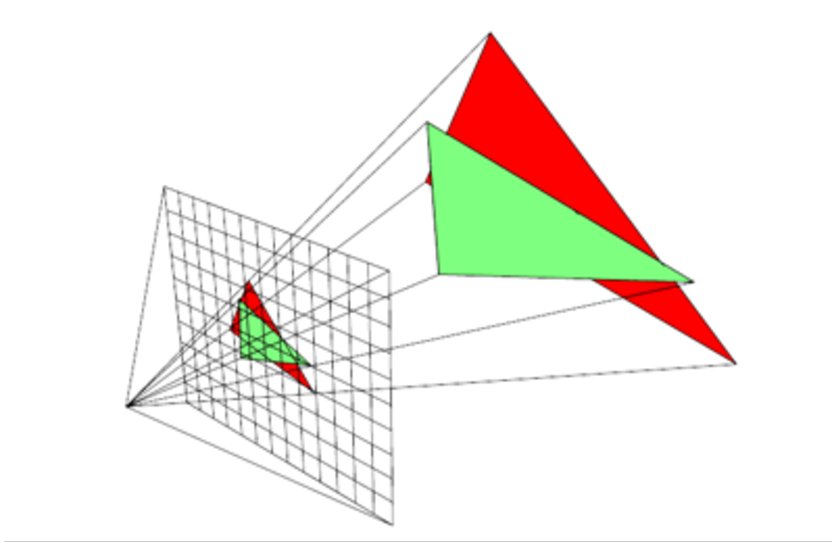
\includegraphics[width=0.47\textwidth]{rasterization.pdf}
  \hspace{\fill}
  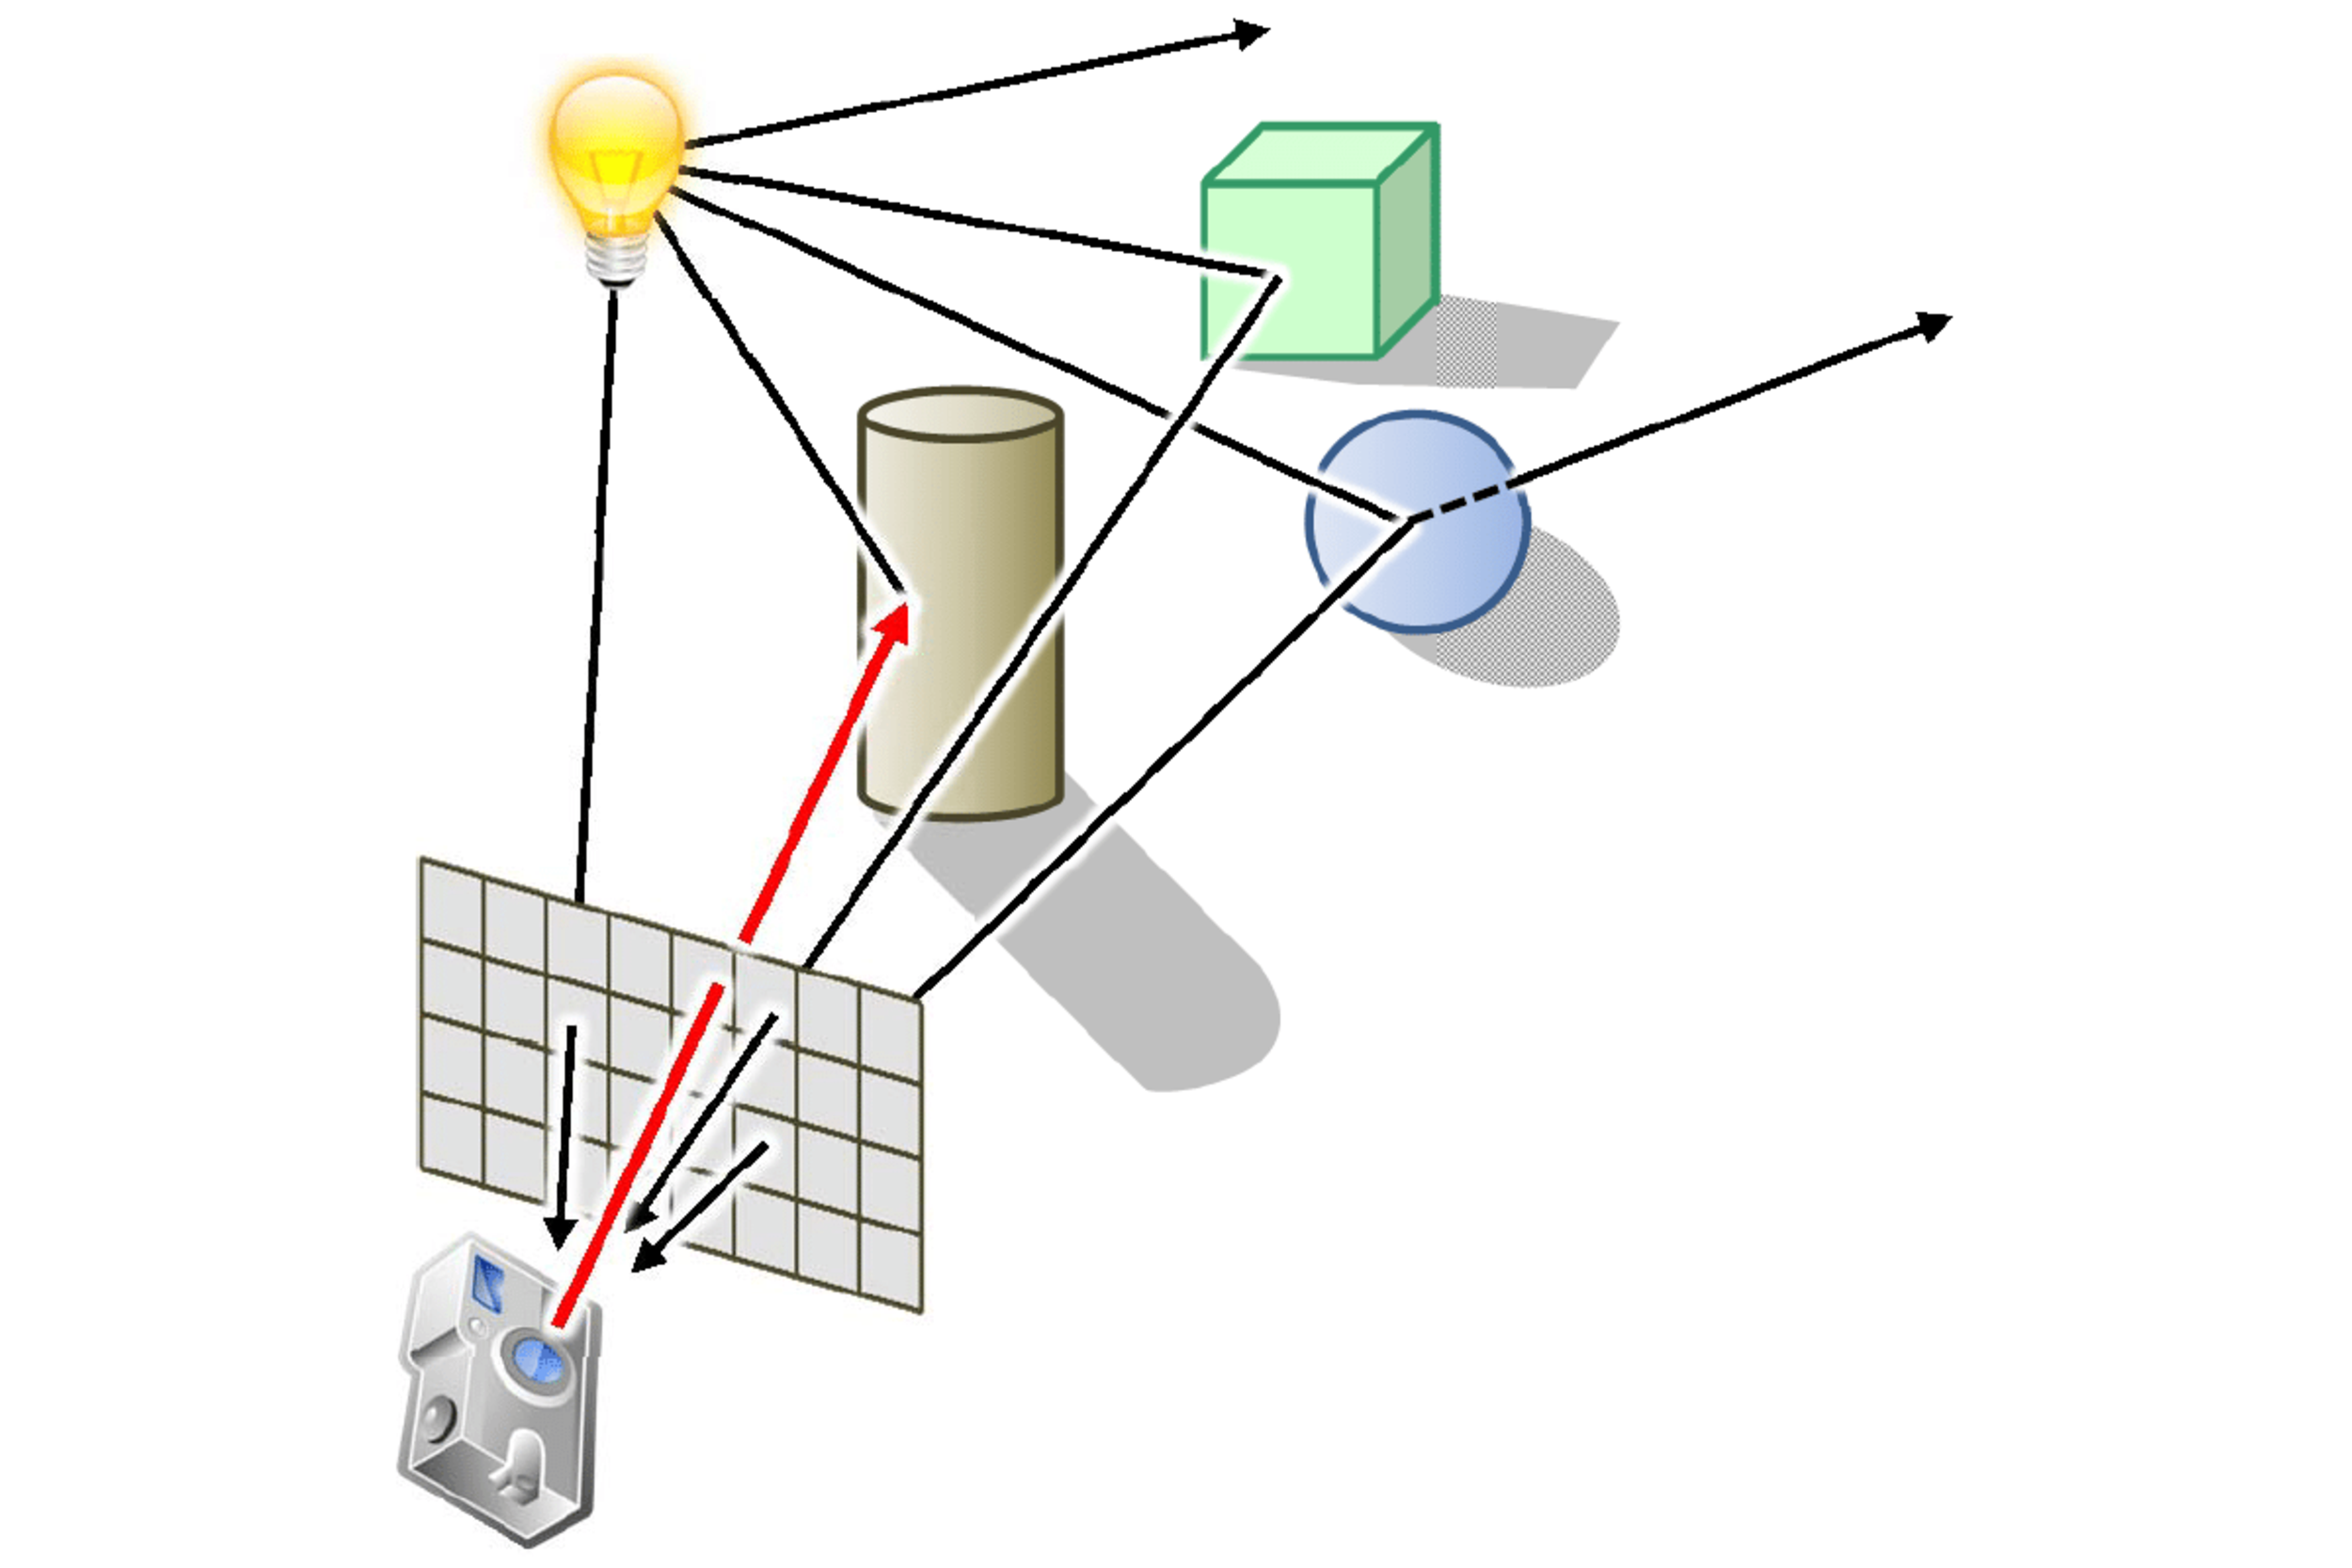
\includegraphics[width=0.47\textwidth]{raytracing.pdf}
  \caption{光栅化和光线追踪示意图}
  \label{fig:rasterization}
\end{figure}

与渲染相对应,逆渲染也是计算机图形学中的一个重要问题。它的主要目标是从提供的图像中推断出物体和场景的三维结构和材质、光照等。逆渲染和传统渲染是恰好相反的两个问题。传统渲染利用场景的三维几何、材质、纹理和光照信息来模拟光线交互,从而生成给定视角下观察得到的二维图像;逆渲染则致力于从一个或多个二维图像中重建物体或场景的三维几何、材质、纹理和光照信息。

三维重建是指从一组或多组图像中恢复出三维场景的几何结构和外观信息的过程。从描述中可以看出,三维重建和逆渲染是非常近似的两个概念。可以认为,三维重建是计算机视觉领域通常习惯的称呼,而逆渲染则是计算机图形学领域的术语。也由于这个区别,三维重建通常更关注物体和场景几何信息的恢复,以及视觉效果上的逼真程度,而逆渲染更注重更为底层的材质和光照信息。

由于三维重建和逆渲染问题的重要性,目前已经存在丰富多样的三维重建算法。主流的重建算法大致可以分为两类:基于视觉几何的传统三维重建和基于深度学习的三维重建。

传统的三维重建主要通过多视角的图像对采集数据的相机位姿进行估计,在通过图像提取特征后,借助深度估计等技术完成从二维图像到三维物体的转换。传统的三维重建算法包括 SfM \cite{SfM}、COLMAP \cite{COLMAP1,COLMAP2} 等。

深度学习出现后,大量将其应用于三维重建的算法也纷纷涌现。有些算法将深度学习和传统三维重建结合,改进传统算法中的某些模块,例如 DeepVO \cite{DeepVO}、BA-Net \cite{BA-Net} 等。更多工作则是直接通过深度学习进行三维重建。NeRF \cite{nerf} 将神经辐射场和体渲染相结合,对三维空间中的色彩和密度进行隐式建模,从而实现高质量的新视角合成。3D Gaussian Splatting \cite{3DGS} 是一种基于体素的三维重建方法,并借助可微光栅化,控制每一个体素对应 3D Gaussian 的形状和大小,实现对三维场景的重建。由于深度学习方法重建质量高、效果好,很快成为了三维重建领域的主要研究方向,神经辐射场和 Gaussian splatting 也很快成为了三维重建中的主要表示形式。

\begin{figure}[htbp]
  \centering
  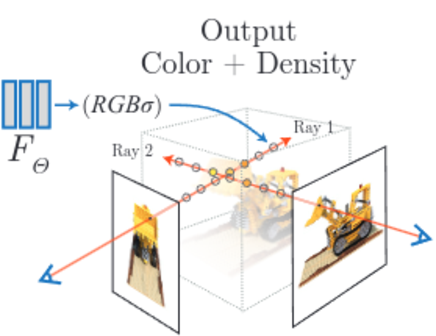
\includegraphics[width=0.47\textwidth]{nerf.pdf}
  \hspace{\fill}
  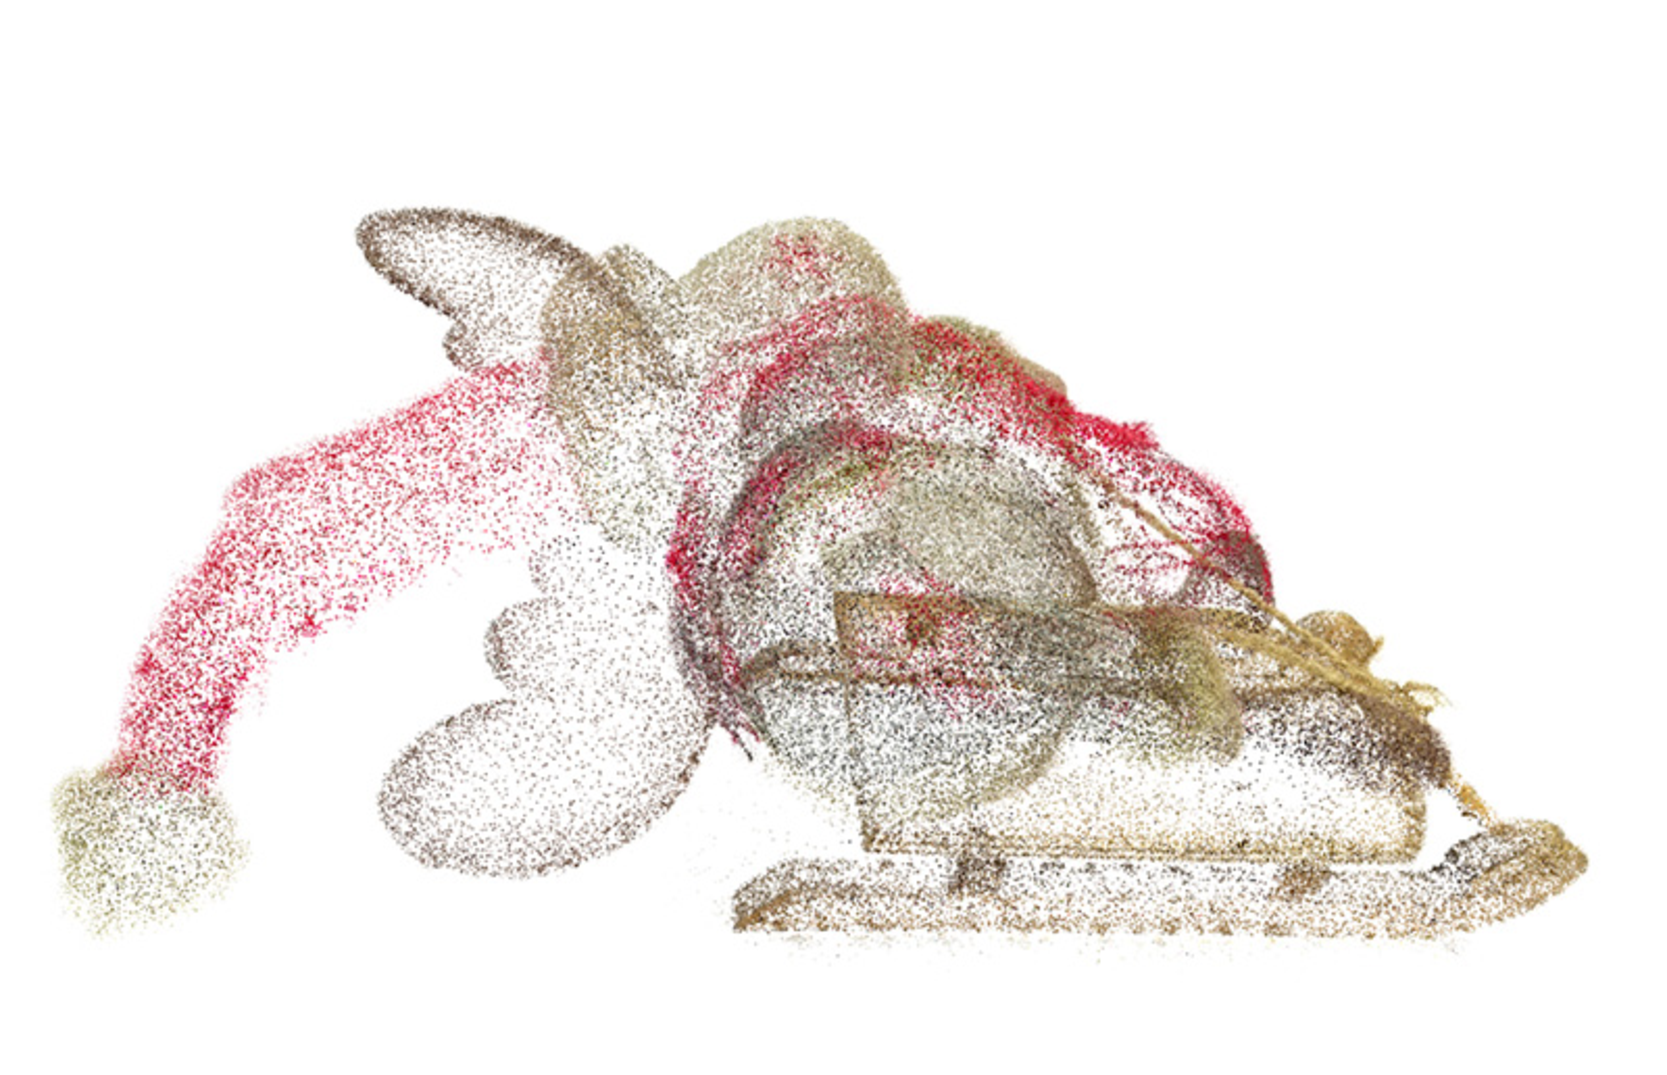
\includegraphics[width=0.47\textwidth]{3dgs.pdf}
  \caption{NeRF 和 3DGS 示意图}
  \label{fig:nerf-3dgs}
\end{figure}

如图 \ref{fig:nerf-3dgs},左图代表 NeRF,右图代表 3D Gaussian splatting。NeRF 采用神经辐射场和体渲染,而3D Gaussian splatting则通过空间中一系列椭球形三维高斯来模拟整个场景。

然而,这些方法也存在问题。无论是神经辐射场或是三维高斯,都属于隐式的几何建模,和传统的显示三维网格(mesh)表示形式有着较大的区别。我们可以通过隐式表示得到漂亮的视觉效果和高质量的新视角合成,但无法得到物体的精确几何信息,不利于下游任务。因此,许多后续工作致力于将这些隐式建模转换为显示的三维网格表示,例如 nvdiffrec \cite{nvdiffrec}、Nerf2Mesh \cite{Nerf2Mesh} 等等。

另一个重要的问题在于如何还原精确的材质和光照信息。NeRF 等一系列相关工作都致力于新视角合成问题,能够在新颖视角下生成极其真实的图像。然而,NeRF 采用的体渲染方法将材质和光照信息烘焙在神经辐射场中,并没有提取显式的材质和光照表示。一些工作尝试通过额外的网络结构来还原材质和光照信息,例如 TensoIR \cite{tensoir} 在 TensoRF \cite{tensorf} 的基础上,通过多层感知机(MLP)从外观特征中提取材质信息,并通过基于物理的可微渲染,在更新密度场的同时更新材质和光照。然而,这些工作大多使用可微光栅化或是简化版的光线追踪,并通过一些额外网络来拟合间接光照。这就导致了他们不能准确地计算全局光照的效果,也不能真实的还原光线和物体或场景的交互。

此外,逆渲染问题本身也是一个不适定(ill-posed)问题。对于给定的单张图像,可能存在多组场景参数与之对应。当输入多张不同角度的图像时,逆渲染问题的解可能会更加稳定,但不适定性仍然存在。一个经典的问题是对于阴影的处理。常见图像的 RGB 空间都是在区间 $[0, 255]$ 中的整数,离散的颜色值意味着在渲染时需要进行取整或截断。而黑色阴影部分对应的 RGB 值太小,可能导致严重的信息丢失。在不使用光线追踪的情况下,我们无法准确地模拟阴影的效果,这就导致许多逆渲染方法会在重建的材质中出现照明伪影。也有一些工作尝试去除这些伪影,例如 SIRe-IR \cite{SIRe-IR} 针对强光环境下的伪影问题,通过同时建模间接辐射场、法线、可见性和直射光,消除材质中的阴影和间接照明,而不会对场景施加严格的约束。但通过可见性来处理伪影的方法仍旧不如光线追踪来得直接有效和准确,并且通过球形高斯来模拟直接和间接光照并不能很好地处理各向异性材质,因此他们无法将金属材质引入考虑范围。

然而,将光线追踪引入三维重建和逆渲染也存在不少困难。想要通过神经网络优化的关键条件是能够计算梯度,而在光线追踪中,我们很难计算渲染结果关于几何的梯度。这是因为光线和物体相交与否是一个不连续的过程,我们难以处理在物体边界处的情形。现有的可微光线追踪方法主要致力于如何计算渲染结果关于几何梯度,并通过神经网络训练优化场景的各个参数。但这些方法大多只能调整三维几何形状的位置大小,而不能生成和删除几何网格,因而往往需要一个合适的几何初始化。但光线追踪可以帮助我们准确地模拟全局光照效果,从而消除重建的材质中的照明伪影,得到更真实的纹理和材质信息。因此,将其引入三维重建和逆渲染中,是一个困难但有意义的任务。

\section{研究内容}

由于可微光线追踪难以处理几何梯度,本文试图通过结合现有的三维重建方法,结合可微光栅化和可微光线追踪,在良好几何结构的基础上,通过光线追踪优化材质和环境照明,以期减少重建的材质中的照明伪影,得到更真实的纹理和材质信息。总的来说,本文的贡献如下:

1. 与现有的逆渲染方法不同,我们的模型重建了一个高质量的水密流形三维网格;

2. 我们的模型同时优化几何、纹理和光照,生成的结果可以方便地应用于下游任务,如重新照明、物理模拟、材质编辑等;

3. 我们的模型同时利用可微分光栅化和可微分光线追踪,恢复了接近现实的材质和光照信息。这种方法有效地减少了材质和纹理中次要光照的照明伪影。

\section{论文组织结构}

本文的结构将按照如下顺序组织:

第二章:相关工作。介绍当前主流的三维重建和逆渲染方法,以及可微光线追踪方法。

第三章:研究方法。详细阐述我们的逆渲染框架和流程,包括 TensoIR 的训练、可微光栅化和可微光线追踪的设计。

第四章:实验结果。首先介绍本文实验采用的数据集和评价标准,以及实验环境和设置,然后展示实验结果和分析,证明第三章介绍的方法的有效性。

第五章:总结和展望。总结本文的工作,指出存在的问题和不足,并展望未来的研究方向。

% !TeX root = ../thuthesis-example.tex
\chapter{相关工作}

\section{神经场表示}

与先前的三维网格、体素、点云的表示形式完全不同,神经场表示是三维几何表示方式的一个卓越革新,预示着三维内容生成和建模的范式转变。这一表示形式在2019年开始被发掘,并且很快成为热门。2021年发表的综述 Neural Fields in Visual Computing and Beyond \cite{neural_field_summary} 中对相关工作进行了总结整理,如图 \ref{fig:neural_field_pub} 所示,两年中已有近300篇工作使用了这一新兴表示。

\begin{figure}
  \centering
  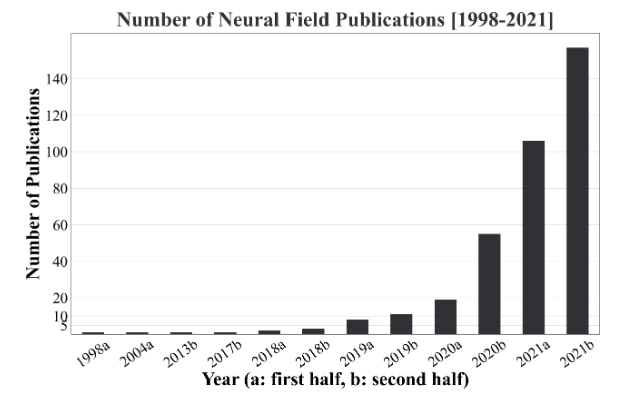
\includegraphics[width=0.9\linewidth]{neural_field_pub.png}
  \caption{神经场相关论文的发表情况}
  \label{fig:neural_field_pub}
\end{figure}

在视觉计算中,典型的神经场算法如下进行:在空间-时间范围内,我们对坐标进行采样,并将采样得到的坐标输入神经网络产生场量。场量的选取与我们的问题所需相对应。然后,我们用正向映射将场量重建为所需内容(例如RGB图像)。最后,我们通过重建信号与传感器收取到的真实信息(例如真实RGB图像)进行比较来计算重建误差和损失,从而引导神经网络的优化过程。

在一系列相关工作中,神经辐射场(NeRF)\cite{nerf} 是最具代表性的方法之一。他成功地将神经场表示引入到三维重建问题中,并且取得了很好的效果,并被广泛应用于新视角合成等问题,沿用至今。因此接下来我们将对其展开介绍。

\subsection{神经辐射场(NeRF)}

神经辐射场的核心在于其场量表示。如下所示:
\begin{equation}
  F(\mathbf{x},\mathbf{d})\to(\mathbf{c},\sigma),
\end{equation}

其中 $\mathbf{x}=(x,y,z)$ 代表三维空间中的坐标,$\mathbf{d}$ 表示视角。输出部分的 $\mathbf{c} = (r,g,b)$ 表示颜色,$\sigma$ 表示密度。$F$ 通常用多层感知机(MLP)来近似。值得注意的是,$\sigma$ 仅是关于 $\mathbf{x}$ 的函数,以此来保证多视角下的一致性,而颜色 $\mathbf{c}$ 同时依赖于位置 $\mathbf{x}$ 和视角 $\mathbf{d}$。

重建过程采用体渲染。在实际物理过程中,光线从光源出发,经过物体表面反射后到达相机。由于光路可逆,我们可以假定从相机处射出光线。对于每一条从相机处发出的光线,我们通过均匀采样或其他采样方法,生成一组采样点,并根据体渲染的渲染公式计算出像素对应的颜色。设相机光线 $\mathbf{r}(t)=\mathbf{o}+t\mathbf{d}$,其中 $\mathbf{o}$表示相机位置,$\mathbf{d}$表示光线方向,则该像素对应的颜色按照下式计算:
\begin{equation}
  C(\mathbf{r})=\int_{t_n}^{t_f}T(t)\sigma(\mathbf{r}(t))\mathbf{c}(\mathbf{r}(t),\mathbf{d}) \mathrm{d}t , \ \mathrm{where} \ \ T(t)=\exp\left(-\int_{t_n}^t\sigma(\mathbf{r}(s))ds\right).
\end{equation}

我们通过采样来估计这个积分。以均匀采样为例,我们在区间 $[t_n,t_f]$ 上采样 $N$ 个点:
\begin{equation}
  t_i\sim\mathcal{U}\bigg[t_n+\frac{i-1}{N}(t_f-t_n), t_n+\frac{i}{N}(t_f-t_n)\bigg],
\end{equation}
并用这些样本来估计 $C(\mathbf{r})$:
\begin{equation}
  \hat C(\mathbf{r})=\sum_{i=1}^NT_i(1-\exp(-\sigma_i\delta_i))\mathbf{c}_i , \ \mathrm{where} \ \ T_i=\exp\left(-\sum_{j=1}^{i-1}\sigma_j\delta_j\right).
\end{equation}

虽然许多神经场表示方法将三维几何形状表示为如上的密度场,但近期有符号距离场(SDF)也开始被广泛使用。有符号距离场可以方便地表示几何形状的边界,因此可以导出三维网格表示,这是密度场所无法做到的。然而,这一转化也导致了渲染质量的显著降低。我们的工作通过将密度场转化为SDF场,再将SDF场转化为高质量连续曲面网格,并通过可微渲染保证了渲染质量。这种转换不仅确保了出色的渲染质量,还拓展了后续下游应用的范围。此外,导出三维网格表示与相应的材料、纹理和光照,使其不再借助神经场表示和神经网络,而是可以直接应用在渲染器中,加速了渲染速度。

\section{可微渲染}

如前所述,渲染是从三维场景得到二维图像的过程。可微渲染则是指这一过程是可微的,即我们可以计算渲染结果对输入场景的梯度,其中输入场景一般包括几何、材质和光照等信息。可微渲染在计算机图形学和计算机视觉中有着广泛的应用,例如图像生成、三维重建、逆渲染等问题。传统渲染管线一般并不可微,主要原因是光线与物体表面的交互是不可导的。因此,可微渲染的一般思路一般是在传统渲染管线中引入可微的近似方法,或者更改渲染算法的某些部分使其可微。本文主要涉及到可微光栅化和可微光线追踪,因此下面对这两个方向的相关工作进行介绍。

\subsection{可微光栅化}

可微光栅化是可微渲染中的重要方法,相关的研究也相对深入。它在传统渲染技术和现代深度学习之间搭建了新的桥梁。可微属性使得网络能够直接从图像数据中学习并优化几何属性,从而端到端地完成三维重建和逆渲染任务。可微光栅化主要目的在于提升性能,它们以局部光照为前提,着色时仅考虑局部阴影,重点在于强调获得有用的可见性梯度,以通过梯度下降优化几何形状。

Shichen Liu 等人提出了 Soft Rasterizer \cite{softraster}。这个工作将确定性的渲染过程看做一个”软“的概率过程。传统的光栅化过程中,对于每个像素,仅选择最上层的三角形片元进行着色。而在 Soft Rasterizer 中,我们将每一个三角形都视作概率云,每一层的三角形都对最终颜色有一定概率贡献。他们提出了一种可微聚合函数,根据概率图和三角形的相对深度融合每个三角形的颜色图,形成最终的渲染结果。这种新的渲染方法使得他们可以将梯度回传到每一层三角形上,包括在传统光栅化意义下被遮挡的三角形。

Soft Rasterizer通过修改传统渲染方法使其变得可微。与之不同,OpenDR \cite{OpenDR} 并没有对前向渲染算法做出任何修改,而是通过在反向传播过程中近似计算梯度来解决该问题。它将像素分为内部像素、边界像素和多边界像素三类分别进行处理,并将图像颜色的梯度近似为像素颜色的差分。

Nvdiffrast \cite{nvdiffrast} 的目标同样是在不更改传统渲染方法的情况下实现可微光栅化。因此在他们的设定下,对于最终图像没有产生影响的片元,例如由于遮挡或者超出屏幕外的部分,梯度应当为零。他们实现了模块化的框架,主要包含光栅化、插值、纹理过滤和抗锯齿四个部分,通过抗锯齿将边界处的不连续性平滑化,从而可以计算梯度。本文中可微光栅化的部分主要借助 Nvdiffrast 实现。

\subsection{可微光线追踪}

相较于可微光栅化,可微光线追踪相关的研究相对较少。这是因为光线追踪的计算复杂度较高,逆渲染时一般不会考虑光线追踪,而且光线追踪的过程中由于存在很多不可导的操作。由于光线追踪需要光线的多次反射,几何形状的微小改变可能会改变每一次反射的方向,叠加起来就会对整条光路产生巨大的影响。与可微光栅化类似,可微光线追踪的主要思路也是通过近似让计算关于几何形状的梯度成为可能。在这个过程中,我们需要考虑到光线追踪的复杂性,以及如何在保证计算效率的同时保证梯度的准确性。

Tzu-mao Li 等人提出的 redner \cite{DiffMCRT} 将渲染的计算分成平滑区域和不连续区域。对于平滑区域,他们采用传统的面积采样方式,并通过边采样替代面积采样的方式解决边界处场景函数关于参数不可导的问题。

Loubet 等人提出了一种重参数化积分的方式来处理不连续问题 \cite{Loubet}。一般来说,光线追踪需要计算如下积分式:
\begin{equation}
  I=\int_{\mathcal X}f(x,\theta) \mathrm{d}x,
\end{equation}
其中积分区域 $\mathcal X$ 通常是球面。所谓的不可导问题是指 $f(x, \theta)$ 由于边界处可见性的变化关于场景参数 $\theta$ 不可导。Loubet 等人通过在 $\theta$ 的邻域 $U(\theta)$ 内找到一个变换 $T: U(\theta)\times\mathcal Y\to\mathcal X$,使得 $T$ 是可导的,从而将积分转化为:
\begin{equation}
  \int_{\mathcal{X}}f(x,\theta) \mathrm{d}x=\int_{\mathcal{Y}}f(T(y,\theta),\theta) |\det J_T| \mathrm{d}y.
\end{equation}
在这种变换后,采样过程中不连续的位置不再随场景参数变化而变化。这也就解决了不可导问题。

Zhang 等人先后提出了 PhySG \cite{PhySG} 和 IRON \cite{IRON} 两个可微渲染框架。PhySG 仅仅考虑直接光照,并不考虑自遮挡和简介光照。他们用球形高斯对环境光进行建模,用 SDF场表示几何形状,并通过法向量的梯度回传至SDF场上来优化几何表示。IRON 则是PhySG 后的进一步工作,他们继承了PhySG 的 SDF场表示,并通过类似于 redner 的基于边缘感知物理的表面渲染优化各个参数。

在另一个名为 Path-space differentiable rendering \cite{PSDR} 的工作中,作者通过复杂的数学推导,直接在路径空间中考虑路径的微分。他们将路径积分的微分分解为内部项和边界项两部分,并在路径空间中分别使用蒙特卡洛方法进行估计。对于边界项,他们采用了一种完全可微的采样方法,因此其导数计算可以非常精确。但这种方法对单个渲染图像的梯度计算需要数十秒的时间,因而不适合于神经网络的训练。


\section{逆渲染}

如前所述,逆渲染旨在从一张或一组图像中获取对场景的物理属性的理解,包括三维几何信息、材质、光照、纹理等等。由于该问题不适定,大部分逆渲染相关的工作都对光照、形状做出一些假设,甚至给定光照条件,或是结合关于光照、阴影、材质、几何形状等的先验知识。

早期的工作借助大量先验来简化问题。Barron 等人在2015年提出的工作中\cite{SIRS},根据形状、反射率和照明的一组先验,将问题表述为统计推理和优化之一。他们将问题规约成:
\begin{equation*}
  \begin{array}{ccc}\text{maximize}_{R,Z,L}&&P(R)P(Z)P(L)\\\text{subject to}&&I=R+S(Z,L)\end{array}.
\end{equation*}
其中,$R$ 是对数反射图像,$Z$ 是深度图,$L$ 是用球谐函数表示的光照。$S(Z,L)$是一个渲染引擎。$P(R), P(Z), P(L)$ 分别是反射率、形状和光照的先验。他们希望重建的模型尽量符合先验,同时需要符合输入图像。由于使用了大量先验,在此不做赘述,我们仅以形状为例,作者希望重建的形状符合以下几个条件:
\begin{itemize}
  \item 光滑。通过最小化曲率的变化来实现。
  \item 表面法线各向同性。我们希望邻近点的法线方向尽量一致。
  \item 边缘处法线约束。理想情况下,假设相机从垂直方向拍摄,则物体边缘处法线应该与边缘垂直,$z$ 分量为零。
\end{itemize}
通过将这些假设数学化,加入到优化问题中,作者最终得到了一个能够重建物体形状、反射率和光照的优化算法。

与上述工作不同,Zhengqin Li 等人通过建立一个大规模形状材质数据集来获取关于形状和材质的先验,并且提出了新的网络架构整体上解决逆渲染问题 \cite{Learning1image}。通过大规模数据集,他们用不同的方式获取了非常强的先验,从而能从单张图片还原出物体的三维形状和材质。

在计算机视觉中,还有部分工作通过估计深度图来还原三维形状。在 Deep 3D Capture \cite{D3DC} 中,输入的多张图像首先经过深度估计网络得到深度图,根据深度图完成图像的粗对齐。接着,通过编码-解码网络,从图像中提取材质、法线等信息,并且通过估计的深度图结合这些信息得到图像,并与真实图像对比来优化网络。这种方法对深度估计的准确性要求较高,且对于复杂的场景,往往难以得到满意的结果。

还有部分工作专注于简单的材质模型。Chen 等人在2021年的工作中,针对没有纹理的简单物体设计了新颖的逆渲染框架。他们在合成数据和真是图像上都获得了相当精细出色的结果。但除了材质模型的假设之外,他们还有一些其他约束,例如光照和相机的绑定、仅使用点光源等。这也就导致这个工作的应用范围受到限制。

\section{小结}

本章介绍了神经场表示、可微渲染和逆渲染等相关工作。神经场表示作为三维几何表示的一种革新,引领了三维内容生成和建模的新方向。可微渲染在传统渲染技术和深度学习方法之间搭建了桥梁,使得渲染过程可导,有助于端到端的三维重建和逆渲染任务。逆渲染则旨在从图像中推断出场景的物理属性,但可以看到,由于逆渲染问题自身的不适定性,多数方法都做了较强的先验和假设。可微渲染也是逆渲染的重要方法之一,可微光栅化常常作为逆渲染中的重要模块,但可微光线追踪由于计算复杂度较高,较少被应用于逆渲染问题。
目前看来,三维重建和逆渲染还不存在一个通用的解决方案。通过神经辐射场,我们可以得到高质量的视觉效果,但其密度场表示并不适合后续应用。而逆渲染方法同样局限,即使能够得到物体表面的反射率、粗糙度等信息,也无法避免会将照明伪影等信息“烘焙”到材质中。如何将可微光线追踪应用于逆渲染问题,是一个值得深入挖掘的方向。

% !TeX root = ../thuthesis-example.tex
\chapter{水密流形三维网格重建}

针对水密流形三维网格重建问题,本章通过将神经辐射场、可微光栅化和可微光线追踪结合起来,提出了一种新颖的解决方案。在重建高质量的三维网格几何表征的同时,我们通过可微光线追踪辅助,还原高质量的材质信息。

本章将首先对任务进行准确定义,然后介绍所需使用的材质和光照模型,最后对网络中的所有模块进行逐一介绍。

\section{问题描述}

\subsection{水密流形三维网格}

我们要求还原水密流形三维网格的几何表示,这是因为相比于密度场或是其他一些三维网格表示,这样性质良好的表示更有利于后续下游任务的进行。

\textbf{三维网格 (mesh):} 三维网格是由一系列连接的顶点、边和面构成的结构,在计算机图形学和几何建模中用于描述三维对象的形状和结构。在本工作中,我们使用三角形网格,即每个面都是一个三角形。

\textbf{水密 (watertight):} 在三维网格的每条边精确地被两个面共享且不超过两个面的情况下,该网格被称为水密的。

\textbf{流形 (manifold):} 一个流形网格需满足以下条件:(1)每条边连接的面最多为两个;(2)每条边与一个或两个面相交,与一个顶点相连的面以封闭或开放扇形结构组织;(3)面之间禁止相互自相交。图 \ref{fig:nonmanifold} 展示了非流形网格的例子。

\begin{figure}
  \centering
  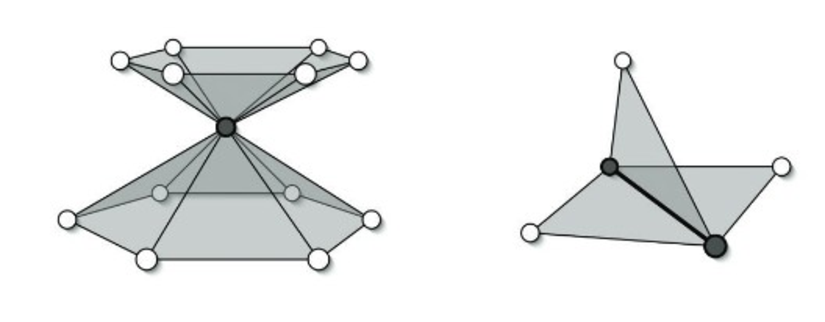
\includegraphics[width=0.8\linewidth]{nonmanifold.pdf}
  \caption{非流形网格示例}
  \label{fig:nonmanifold}
\end{figure}

\subsection{输入}

如上文所述,我们的任务是三维物体的逆渲染。在这个问题中,输入是一系列不同角度所拍摄或渲染的物体图像 $I_1, I_2, \cdots, I_n$,以及相对应的相机位姿参数 $p_1, p_2, \cdots, p_n$。所有图像都是通过相同的相机对同一个物体在固定光照条件下从不同角度进行拍照得到的。我们使用仿真数据来验证我们方法的有效性。

\subsection{输出}
我们模型的输出包含三个部分 $(G, M, L)$。其中 $G$ 代表重建的水密流形三维网格表示,$M$ 代表对应的材质信息,$L$ 则代表光照。

\section{简化的迪士尼原理化BRDF}

我们的模型采用简化的迪士尼原理化BRDF作为着色模型。迪士尼原理化BRDF (Disney Principled BRDF) \cite{DisneyBRDF} 是计算机图形学领域广泛应用的经典着色模型。着色模型的建立是为了准确模拟光照和不同物体表面交互时的不同表现。迪士尼原理化BRDF通过十个参数,能够定义大部分常用表面材质,并且创建逼真且一致的渲染效果。

为了理解着色模型,我们首先需要理解渲染方程:
\begin{equation}
  L_{o}\left(\mathbf{x},\omega_{o}\right) =L_{e}\left(\mathbf{x},\omega_{{o}}\right) +\int_{\Omega}f\left(\mathbf{x},\omega_{{i}},\omega_{{o}}\right)L_{i}\left(\mathbf{x},\omega_{{i}}\right)\cos\theta_{i}d\omega_{{i}},
\end{equation}

其中,$\mathbf{x}$ 指三维空间中的位置,$\omega_i$ 指光线入射方向,$\omega_o$ 指观察方向,$L_o$ 指观察方向的辐射度,$L_e$ 指自发光辐射度,$f$ 指BRDF,$L_i$ 指入射方向的辐射度,$\theta_i$ 指入射方向与法向的夹角。积分域 $\Omega$ 一般是表面法线所对应的半球。我们所说的着色模型主要就是上式中的 $f$ 函数,它接收入射方向和出射方向,返回对应的反射率。

迪士尼原理化BRDF的参数包括漫反射颜色(baseColor)、次表面(subsurface)、金属度(metallic)、高光度(specular)、粗糙度(roughness)、各向异性度(anisotropic)等,其中大部分参数是为了某些特定的材质服务,例如专门为了模仿一些纺织物布料而设计的 sheen 参数。在我们的模型中,为了简便,对迪士尼原理化BRDF做了一些简化,仅保留三项参数:漫反射颜色(baseColor)、粗糙度(roughness)、金属度(metallic)。其中漫反射颜色决定了材质的底色,其余两项参数对物体材质的影响如图\ref{fig:brdf}。
\begin{figure}
  \centering
  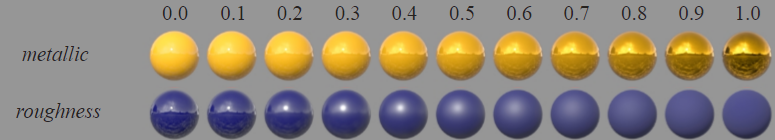
\includegraphics[width=\linewidth]{brdf.png}
  \caption{迪士尼原理化BRDF的两个参数对物体材质的影响}
  \label{fig:brdf}
\end{figure}

\newpage
简化后的 BRDF 函数可以分为漫反射和金属反射两部分。漫反射的BRDF计算公式如下:
\begin{equation}
  f_{\text{Diffuse}} = \frac{\text{baseColor}}{\pi}F_{D}(\omega_{\text{in}})F_{D}(\omega_{\text{out}})|n\cdot\omega_{\text{out}}|,
\end{equation}
其中
\begin{align}
  F_{D}(\omega) &=\begin{pmatrix}1+(F_{D90}-1)(1-|n\cdot\omega|)^5\end{pmatrix}, \\
  F_{D90} &=\frac12+2\cdot\mathrm{roughness}\cdot|h\cdot\omega_{\mathrm{out}}|^2.
\end{align}
金属反射部分的BRDF计算公式如下:
\begin{equation}
  f_\mathrm{metal}=\frac{F_mD_mG_m}{4|n\cdot\omega_\mathrm{in}|},
\end{equation}

其中
\begin{align}
  F_{m} &= C_0+\left(1-C_0\right)\left(1-(h\cdot\omega_{\mathrm{out}})\right)^5,\\
D_{m} &= \frac {\alpha ^ 2} {\pi \left(\mathrm{NoH}^2 (\alpha^2 - 1) + 1\right)^2}, \\
G_{m} &= G(\omega_{in}) G(\omega_{out}),\\
C_0 &= \mathrm{metallic}\cdot\mathrm{baseColor},\\
\alpha &= \max (\mathrm{roughness}^2, 0.0001),\\
\mathrm{NoH}&= \cos (\left<h, n\right>) = h \cdot n,\\
G(\omega) &= \frac 2 {\sqrt{\frac {\alpha^2} {(\omega \cdot n)^2} + 1 - \alpha^2 }+1}.
\end{align}

我们将上述两个部分综合起来得到最终的 BRDF 函数表达式:
\begin{equation}
  f_{\mathrm{final}}=(1-\text{metallic})\cdot f_\text{diffuse}+f_\text{metal}.
\end{equation}

\section{模型设计}

我们的模型流程如图\ref{fig:pipeline}。首先,我们会通过修改版的 TensoIR\cite{tensoir} 得到一个密度场和对应的材质、光照等信息。其次,我们会通过可微 Marching Cube 将三维密度场转换成三维网格表示,同时通过可微光栅化重新优化材质、光照信息,以使其与三维网格表示相匹配。最后,我们通过可微光线追踪技术,固定三维网格表示,优化材质、光照信息,以去除重建的材质中的照明伪影,从而得到更真实的纹理和材质信息。下面我们将对三个部分逐一进行介绍。

\begin{figure}
  \centering
  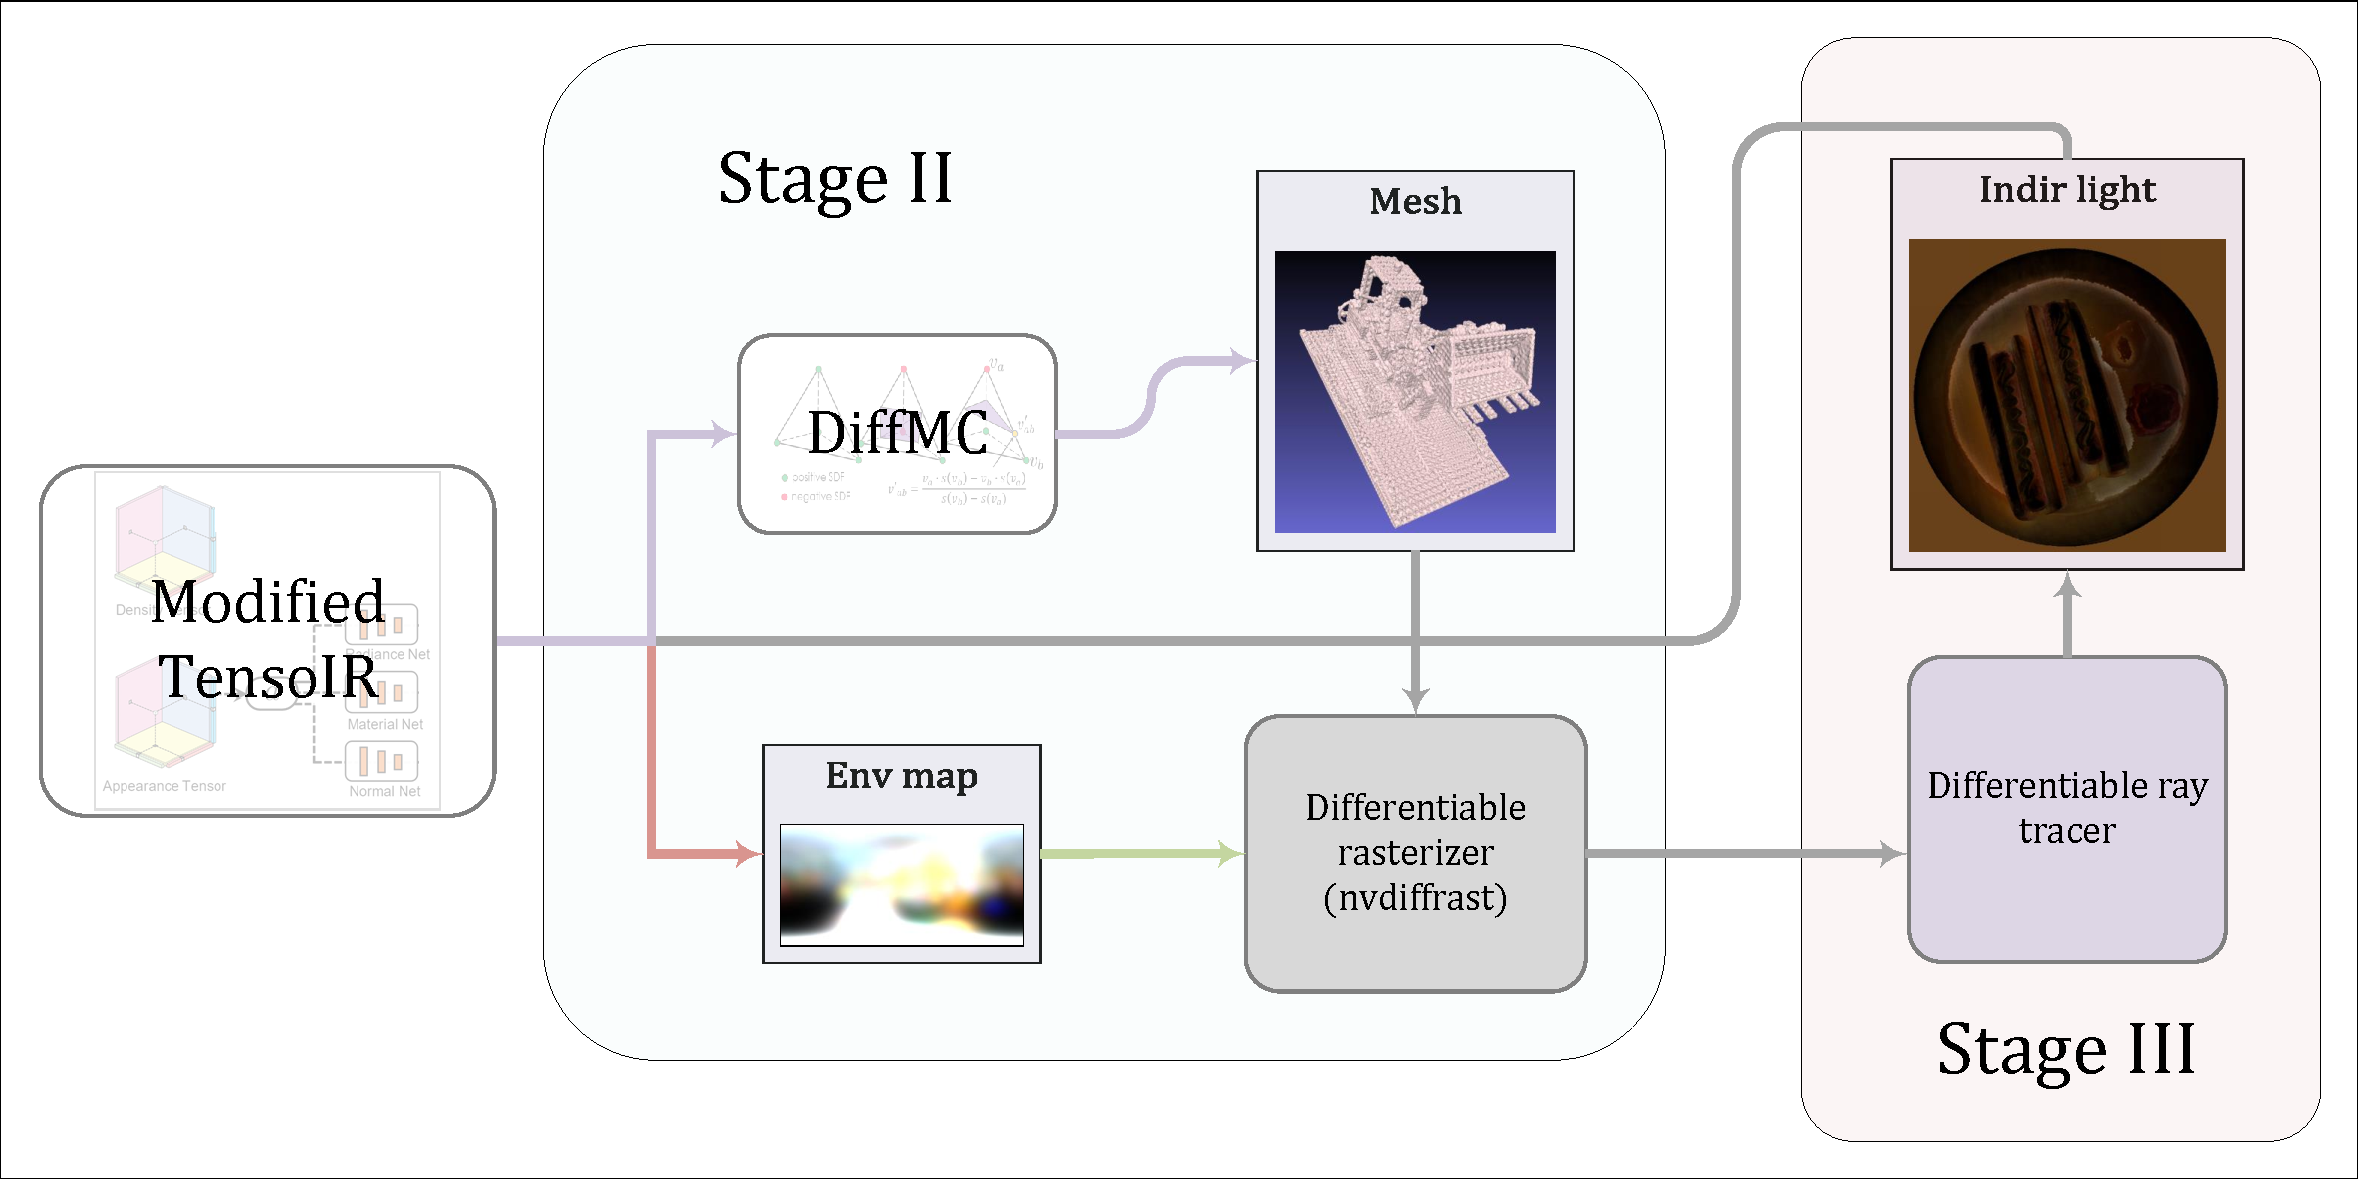
\includegraphics[width=0.7\linewidth]{pipeline.pdf}
  \caption{模型分阶段流程图}
  \label{fig:pipeline}
\end{figure}

\subsection{第一阶段:修改版 TensoIR}

TensoIR 是一个基于神经网络和深度学习的逆渲染框架,由金和刘等人在2022年提出 \cite{tensoir}。该模型在合成和真实数据上都取得了当时的最好效果。它的核心思想在于用 NeRF 中体渲染的方式模拟间接光照,并以此替代路径追踪中的多次迭代,从而实现快速的优化材质信息。它的输入是一系列不同角度所拍摄或渲染的物体图像 $I_1, I_2, \cdots, I_n$,以及相对应的相机位姿参数 $p_1, p_2, \cdots, p_n$。在 TensoIR 中,我们需要同时优化密度场 $D$、外观网络 $a$ 以及环境光照 $L$。TensoIR 的流程如图\ref{fig:tensoir}所示。

TensoIR 的场表示借助了 TensoRF \cite{tensorf} 的表示形式,我们以密度场为例来说明这个表示形式。密度场可以视作函数 $D: \mathrm{R} ^3 \to \mathrm{R}$,输入是三维空间中的位置,输出是一个实数代表密度值。除了用神经网络模拟该函数之外,我们也可以用传统的方式,在三维空间中离散采样,并通过插值计算出任意位置的密度值。假设我们在 $[-1,1]^3$ 的立方体内做均匀采样,我们需要 $O(n^3)$ 的采样点数($n$ 为每个坐标轴上的采样数),这会耗费太多的空间。因此在 TensoRF 中,作者提出了 VM 分解和 CP 分解来解决这个问题。VM 分解是 TensoRF 和 TensoIR 中最终采用的分解方式,因此下面仅对其展开介绍。

\begin{figure}[h]
  \centering
  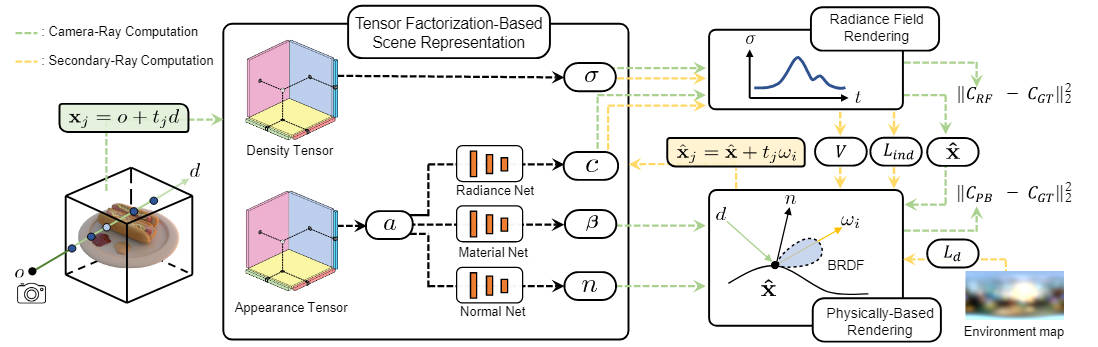
\includegraphics[width=\linewidth]{tensoir.jpg}
  \caption{TensoIR 模型流程图}
  \label{fig:tensoir}
\end{figure}

VM 分解的核心思想在于将三维向量场分解为一维向量和二维矩阵的乘积。具体来说,用 $\mathcal{T}$ 表示三维向量场,我们按照下式进行分解:
\begin{equation}
  \mathcal{T}=\sum_{r=1}^{R_1}\mathbf{v}_r^1\circ\mathbf{M}_r^{2,3}+\sum_{r=1}^{R_2}\mathbf{v}_r^2\circ\mathbf{M}_r^{1,3}+\sum_{r=1}^{R_3}\mathbf{v}_r^3\circ\mathbf{M}_r^{1,2}.
\end{equation}

其中,$\mathbf{v}_r^i$ 是一维向量,$\mathbf{M}_r^{j,k}$ 是一个 $n_j \times n_k$ 的矩阵。这样,我们就将三维向量场分解为了三个部分,每个部分都是一个一维向量和一个二维矩阵的乘积。这样的分解方式使得我们可以用 $O(n^2)$ 的参数量来表示三维向量场。这样分解的坏处在于降低了向量场的表示能力,但是在实际应用中,我们发现 VM 分解的表示能力已经足够应对绝大部分情况。而相较于神经网络,这样的表示方式更为简洁、直接,并且计算效率更高。

如图 \ref{fig:tensoir} 所示,TensoIR 通过上述的表示方式,同时表征密度 $\sigma$,颜色 $c$,BRDF 参数 $\beta$ 和法向方向 $n$。其中,BRDF 参数 $\beta$ 包含两部分,分别是漫反射率 $\alpha = \mathrm{MLP}_{\mathrm{albedo}}(\beta)$ 以及表面粗糙度 $r=\mathrm{MLP}_{\mathrm{roughness}}(\beta)$。根据这些参数,他们得以同时进行神经辐射场渲染和基于物理的渲染,并同时对上述所有参数进行优化。在基于物理的渲染中,他们对渲染方程做出了改动:
\begin{equation}
  L_{\mathrm{i}}(\mathbf{\hat{x}},\omega_{i})=V(\mathbf{\hat{x}},\omega_{i})L_{\mathrm{d}}(\omega_{i})+L_{\mathrm{ind}}(\mathbf{\hat{x}},\omega_{i}),
\end{equation}
其中 $V$ 是可见性函数,$L_{\mathrm{d}}$ 是直接光照,$L_{\mathrm{ind}}$ 是间接光照。我们用神经辐射场模拟间接光照,即:
\begin{equation}
  L_{\mathrm{ind}}(\mathbf{\hat{x}},\omega_i)=C_{\mathrm{RF}}(\mathbf{\hat{x}},\omega_i).
\end{equation}

在我们的模型中,由于所需参数不同,我们对 BRDF 参数 $\beta$ 做了一些改动。在 3.2 节中提到,我们的着色模型需要漫反射颜色(baseColor)、粗糙度(roughness)、金属度(metallic)三个参数。因此我们通过三个不同的多层感知机来分别预测这三个参数,并根据这些参数进行着色和基于物理的渲染。

关于环境光照,我们假设其为一个球形高斯混合模型,即 $L(\omega) = \sum_{i=1}^k w_i \mathcal{N}(\mu_i, \Sigma_i)$,其中 $\omega$ 是光线的方向,$w_i$ 是权重,$\mu_i$ 是均值,$\Sigma_i$ 是协方差矩阵。后续的可微光栅化和可微光线追踪也都会使用这个光照模型。

由于 TensoIR 同时通过神经辐射场和物理模型渲染两张图片,与真实图像计算损失函数,并同时优化上述提及的所有参数,它能够提供较为精确的密度场、材质信息和光照信息,可以给后续训练一个很好的初始化。在第一阶段结束后,我们获得了一个较为精准的密度场 $\sigma$,BRDF 参数 $\beta$,法向方向 $n$ 和用球形高斯表示的环境光 $L$。

\subsection{第二阶段:可微光栅化}

在第二阶段中,我们首先通过可微 Marching Cube 将三维密度场转换成三维网格表示,并通过可微光栅化,在一阶段结果的基础上,同时优化几何形状、材质、光照信息。

\subsubsection{可微 Marching Cube (DiffMC) \cite{wei2023neumanifold}}

我们首先通过可微 Marching Cube 将三维密度场 $\sigma$ 可微地转化成三维网格表示。Marching Cube 是一种常用的三维重建算法,然而,传统的 Marching Cube 算法 \cite{MarchingCube} 是不可微的,这使得我们无法直接在神经网络中使用并反向传播梯度。因此,我们需要对 Marching Cube 算法进行改进,使其可微。这里我们直接使用了 Wei 等人实现的可微 Marching Cube 模块。该模块接受有符号距离场作为输入,通过一个可微的前向过程,生成一个水密流形三维网格。在训练过程中,我们可以直接对有符号距离场进行反向传播,从而优化几何形状。

但是在第一阶段中获得的密度场 $\sigma$ 并不能直接作为 DiffMC 的输入,因此我们需要首先将其转换为有符号距离场。我们首先将密度转换为不透明度:
\begin{equation}
  \alpha = 1 - \exp(-\sigma \cdot \delta).
\end{equation}

其中,$\alpha$ 表示不透明度,$\sigma$ 表示密度值,$\delta$ 表示第一阶段 TensoIR 中使用的体渲染的步长。我们设定 $t$ 为一个阈值,当 $\alpha > t$ 时,我们认为该点在物体内部,当 $\alpha \leq t$ 时,我们认为该点在物体外部。我们将有符号距离场定义为:
\begin{equation}
  \text{SDF} = \alpha - t.
\end{equation}

我们将该 $\text{SDF}$ 作为 DiffMC 的输入,并以此得到水密流形三维网格表示 $G$。

\subsubsection{可微光栅化}

在得到三维网格表示 $G$ 后,我们需要将其与 BRDF 参数 $\beta$ 和环境光 $L$ 相结合,渲染出图像,并与真实图像计算损失。

在3.3.2.1 节可微 Marching Cube 中,我们将密度场转换为三维网格表示。这一步骤同样带来了问题。原先的材质信息 $\beta$ 是与密度场 $\sigma$ 和体渲染相对应,但在3.3.2节中,我们需要与新的三维网格表示 $G$ 与光栅化相结合,因此需要重新优化材质信息。但原先的材质信息提供了一个很好的初始化。这是因为如果给定一个准确的密度场 $\sigma^*$ (物体外部密度为 $0$,物体内部密度为$1$)和对应的准确的三维网格表示 $G$,那么通过体渲染和光栅化分别得到的两组渲染图像几乎是相同的。因此,可微 Marching Cube 带来的表示形式的迁移造成的误差本质上是由于密度场的不准确性造成的。而 TensoIR 提供的密度场的误差相对较小,因而我们可以用3.3.1节得到的 BRDF 参数 $\beta$ 作为初始化,通过优化得到更好的材质信息。

我们使用 nvdiffrast \cite{nvdiffrast} 作为可微光栅化器。在渲染时,我们计算各个方向光线与三维网格的表面交点,并用表面法向网络 $n$ 而非根据 $G$ 计算的法向 $n'$ 作为法向信息进行渲染,这是因为 $n'$ 同时也受到密度场不准确的影响。

在这一阶段训练结束后,我们期望得到一组三维网格表示 $G$,以及与之对应的 BRDF 参数 $\beta$,法向网络 $n$以及环境光照 $L$。在这一步结束后我们已经可以导出一个高质量的三维网格表示。但是,由于我们使用的 TensoIR 中的体渲染和第二阶段的可微光栅化都不能很好地处理全局光照,这一步结束后材质中会存在大量照明伪影。因此,我们需要引入第三阶段,通过可微光线追踪来解决这个问题。

\begin{figure}
  \centering
  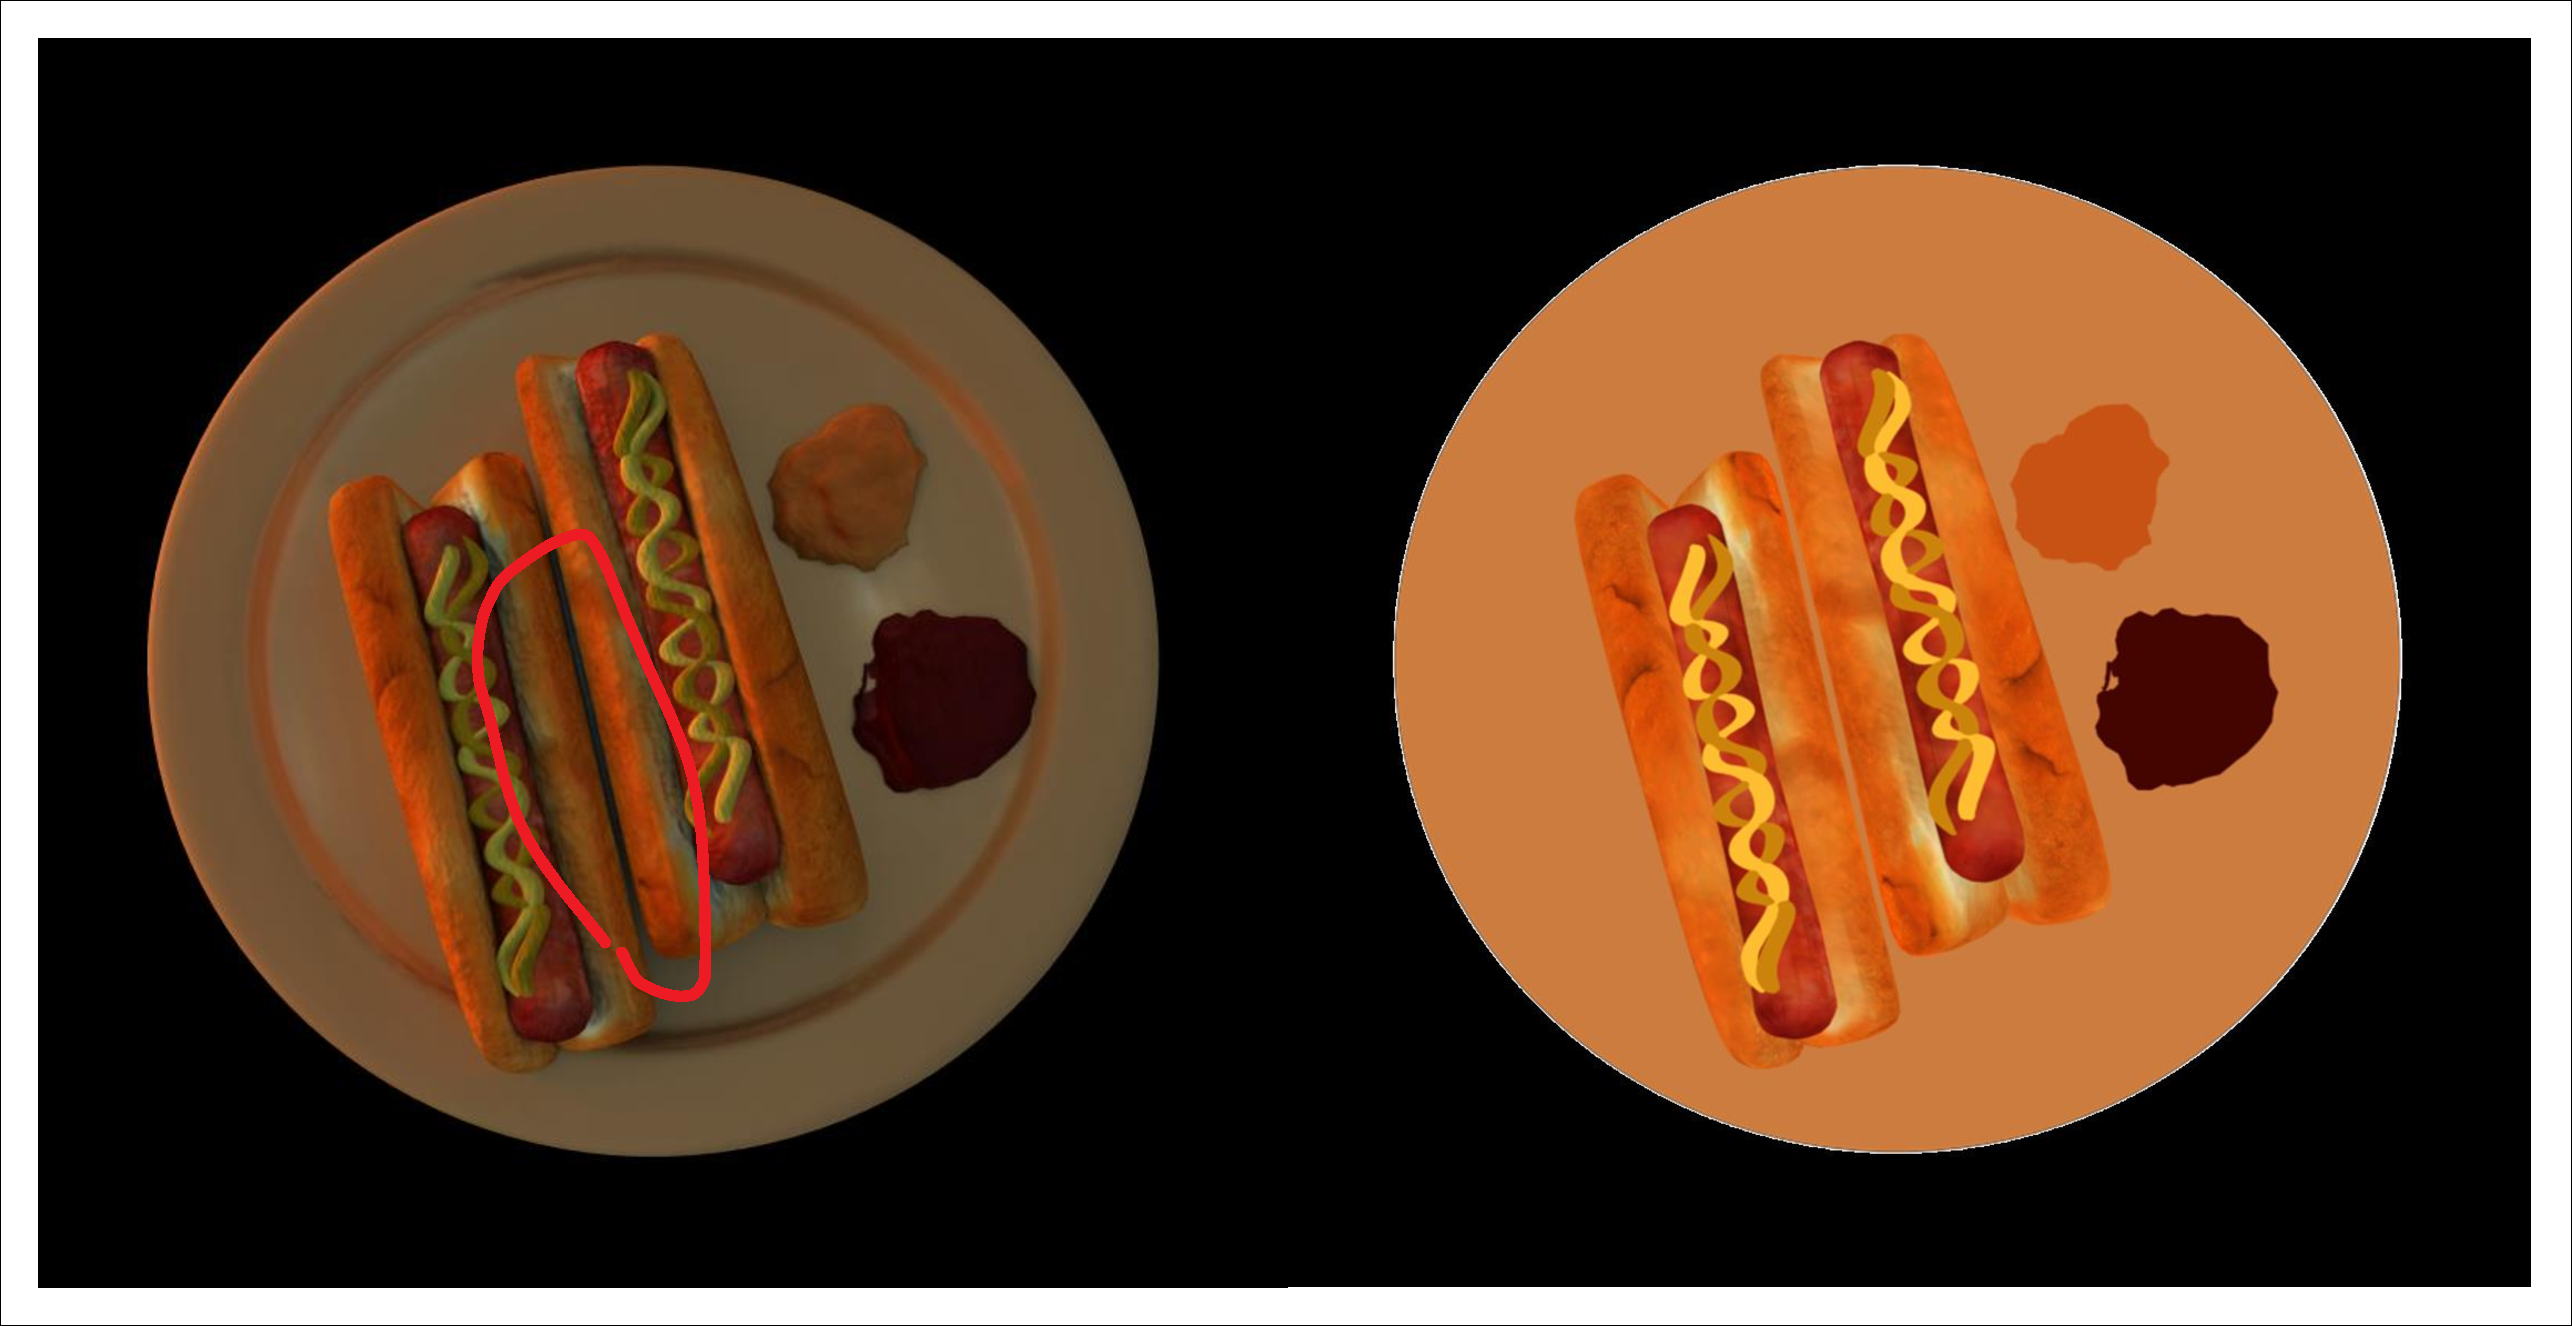
\includegraphics[width=\linewidth]{bakedshadow.pdf}
  \caption{材质中的照明伪影示意}
  \label{fig:bakedshadow}
\end{figure}

如图 \ref{fig:bakedshadow}。左侧是第二阶段训练结束后生成的漫反射颜色图像,右侧是真实的漫反射颜色图像。可以看到,左侧图像红圈内的区域存在照明伪影,呈黑色,这是因为我们的模型无法很好地处理全局光照,因此错误地将阴影所产生的黑色烘焙进材质里。而右侧图像对应位置的颜色与盘子的底色是完全相同的,并没有阴影出现。

\subsection{第三阶段:可微光线追踪}

在第二阶段,我们已经生成了水密流形三维网格 $G$,以及对应的 BRDF 参数 $\beta$,环境光照 $L$。接下来我们引入可微光线追踪来减少材质中的照明伪影。

\subsubsection{原理}

在 2.2.2 节,我们对可微光线追踪进行了介绍,也提到了它的优缺点。我们提到,由于可微光线追踪考虑了全局光照,能够真实准确地模拟光线与物体表面的交互过程。然而,由于计算几何形状梯度的困难性,现有的可微光线追踪方法往往效率低下,渲染一张图片并计算梯度的时间成本很高,不适用于神经网络训练。我们调研了现有的可微光线追踪方法,但都不适合我们的使用场景。具体分析可见附录 \ref{sec:compare}。

注意到,我们已经通过可微 Marching Cube 得到了一个高质量三维网格表示 $G$,因而我们可以固定三维几何表示,优化其余参数。这样,我们也不需要计算最终损失函数关于几何形状的梯度,从而大大简化可微光线追踪。虽然光线追踪中涉及大量的随机采样过程,但在固定几何表示 $G$ 的情况下,从相机位置出发的每一条光路在计算渲染前都是已经确定的。我们只需要根据采样得到的光路,计算每条光路与物体表面交互的过程,并得到渲染图像,整个过程自然是可微的。

\subsubsection{实现}

根据上述原理,我们自己实现了可微光线追踪框架。接下来我们将简要介绍实现细节。

我们的可微光线追踪器 new-renderer,接受场景信息(包括多个物体、对应的材质和环境光照)及光线方向作为输入,输出渲染后的图像。在渲染过程中,由于硬件限制,我们设定每像素采样率 $\text{spp}=128$,光线追踪深度 $\text{depth}=6$。

我们仿照 Mitsuba 的格式用字典储存整个场景。场景中的每个物体都保存为单独的 obj 文件,并在场景字典中通过 to\_world 矩阵指定其在场景中的位置。

我们仿照 pbrt \cite{PBRT3e} 的方式实现渲染器。除了我们模型中需要用到的神经网络材质模型外,为了调试渲染器以及确定渲染器的正确性,我们也实现了额外的材质模型,包括漫反射模型、简化版原理化 BRDF 模型、导体 BRDF。所有的材质模型都封装成统一格式的类,并且提供计算反射率函数值、重要性采样以及计算采样概率的借口。我们也实现了额外的光照模型,包括点光源模型和纯色环境光模型。

我们借助 Mitsuba\cite{Mitsuba3} 库计算光线与物体表面的交点。在后续工作中,我们也考虑自行实现光线与物体表面的交点计算,以减少依赖并提升效率。在这一阶段,我们仍然使用法向网络 $n$ 而非几何形状 $G$ 计算得到的法向作为法向信息进行渲染。这不仅省去了计算几何形状梯度的步骤,保持模型统一性,而且神经网络表示的法向场可以让渲染结果更平滑,不再需要抗锯齿或法线插值等操作。

在第三阶段完成后,我们已经得到了一个高质量的三维网格表示 $G$,以及对应的 BRDF 参数 $\beta$,法向网络 $n$ 和环境光照 $L$。这一阶段结束后,我们期望从材质中去除了部分照明伪影,还原了更真实的漫反射颜色。

\section{训练方法}

最朴素的训练方法是按照阶段顺序依次训练。此外,我们也支持第二、第三阶段的反复训练。第三阶段的目的是去除烘焙在材质中的照明伪影,我们在训练过程中固定了三维几何表示,优化剩余参数。事实上,几何表示的质量和光线追踪的效果息息相关。几何表示与真实几何的差异会导致光线追踪光路的误差,而这种差异在反射次数增加时会被放大。因此,我们也需要在可微光线追踪结束后,通过重新进行可微光栅化训练更新三维网格表示 $G$。反复的迭代可以带来更高质量的重建和逆渲染结果。

% !TeX root = ../thuthesis-example.tex

\chapter{实验结果与分析}

\section{数据集介绍}

本文主要在仿真数据上进行了实验,后续则将会在实验室采集的真实数据集 OpenIllumination\cite{liu2024openillumination} 上进行实验。由于数据对于逆渲染而言非常关键,我们需要在适合的数据集上进行测试。例如,我们的材质模型较为简化,因而无法处理透明物体。此外,我们希望环境光尽量接近自然光,过强和过弱的光源都会给逆渲染带来巨大挑战。前者会导致过分曝光,从而无法判断物体表面的真实颜色,后者则会导致过量阴影。

基于上述原因,我们选择了三维重建领域常见仿真数据集 Nerf-synthetic\cite{nerf} 数据集,并按照我们的需求,将三维场景进行了重新渲染。我们采用了统一的环境光映射,如图 \ref{fig:envmap} 所示。

\begin{figure}
  \centering
  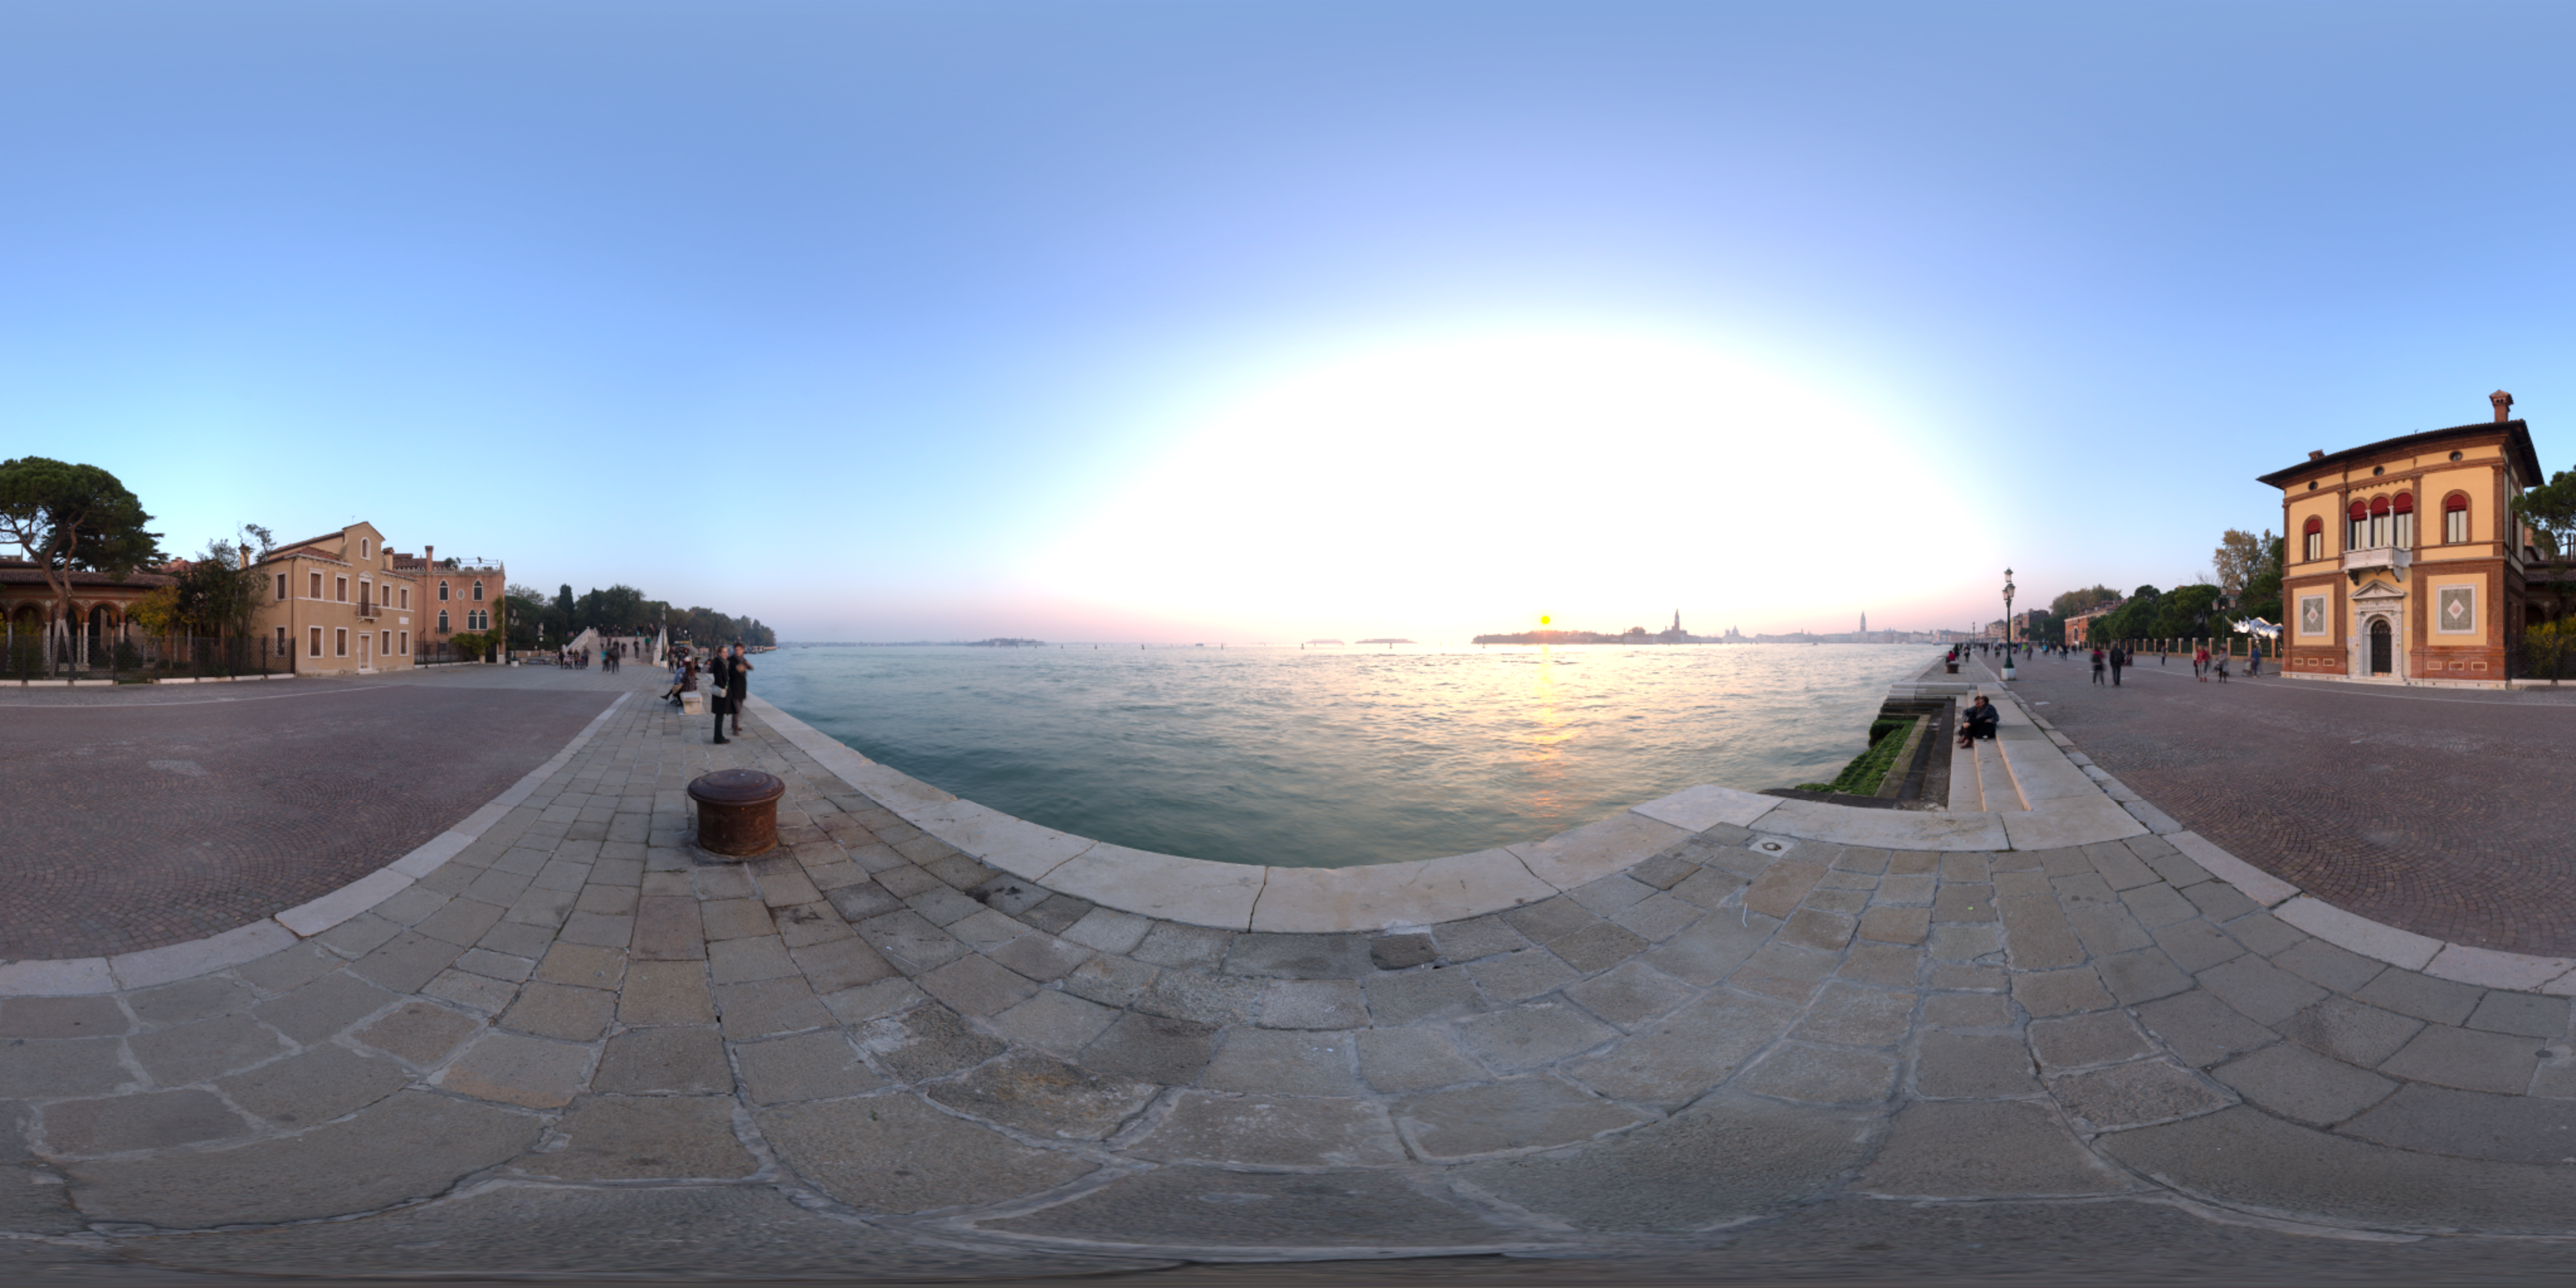
\includegraphics[width=0.8\linewidth]{envmap.pdf}
  \caption{环境光图}
  \label{fig:envmap}
\end{figure}

理论上说,我们期望用我们自己实现的光线追踪器完成数据的渲染过程。这是因为渲染并没有理论上的正确与错误之分,生成数据与训练使用相同的渲染器可以保证渲染过程的一致性,从而尽可能还原真实材质。然而,由于我们的光线追踪器的实现尚未完全,我们暂时使用了 Blender \cite{blender} 进行重新渲染。

Nerf-synthetic 包含八个场景,分别是热狗、材质、植物、乐高、麦克风、鼓、椅子和船。每个场景对应了 400 组相机参数,也即400 个不同视角,按照数据集原始设置,分为训练集、验证集和测试集三个部分,分别包含 100、100 和200组相机参数。渲染图片分辨率为 $800\times 800$。

由于时间限制并考虑到模型本身涉及到的材料、三维几何复杂度等,我们选择了其中的三个模型进行实验,分别是热狗、乐高和植物。这三个模型的复杂度适中,且包含了不同的材质,可以很好地验证我们的模型的有效性。

\begin{figure}
  \centering
  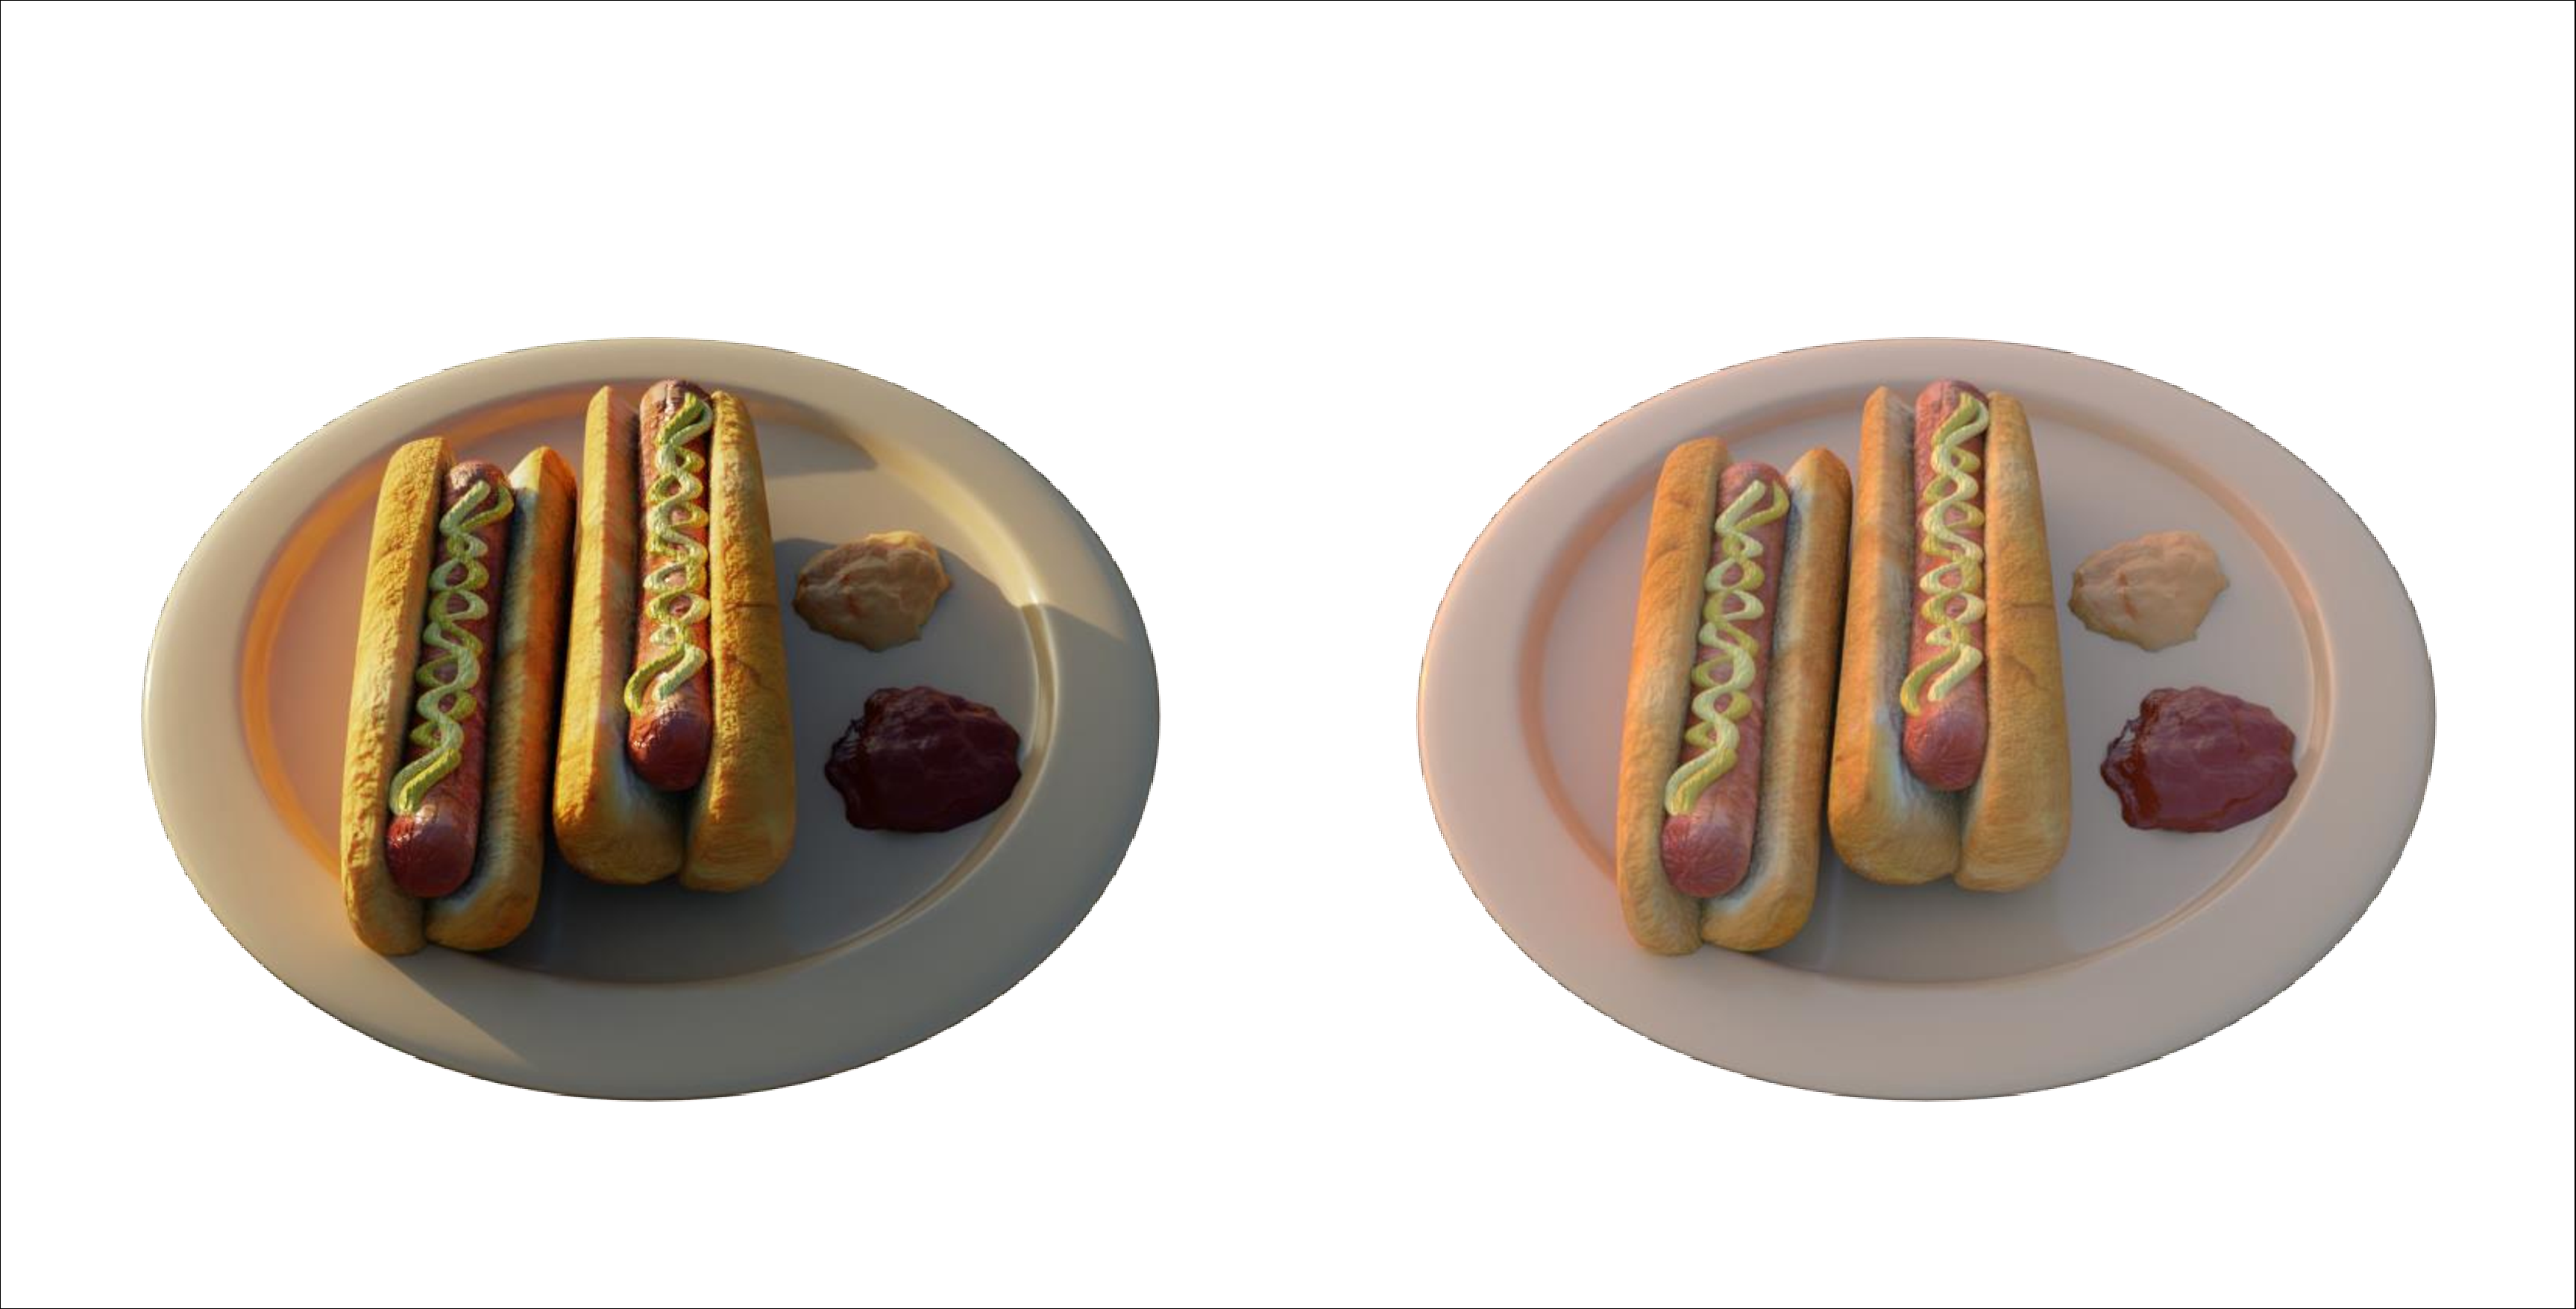
\includegraphics[width=0.8\linewidth]{cmp.pdf}
  \caption{原始数据和我们重新渲染的数据对比}
  \label{fig:cmp}
\end{figure}

图 \ref{fig:cmp} 中展示了原始的 Nerf-synthetic 的原始数据和我们重新渲染结果对比。可以看到,左侧原始数据中有大片的阴影,这对逆渲染并不友好。右侧重新渲染的数据在保留部分阴影的同时,光照更加均匀。

\section{评价指标}

针对我们的任务,我们需要衡量如下几个指标:

\begin{itemize}
  \item 新视角合成的图像质量。新视角合成是三维重建和逆渲染中最常见的任务之一。我们需要根据给定的新的相机参数,合成对应视角下的图像,并与该视角下的真实图像比较。我们通常使用 SSIM 和 PSNR 作为评价指标。
  \item 材质的准确度。我们的模型旨在恢复真实材质信息。因此,我们还将设计新的指标用于评估重建的材质信息与真实材质信息之间的相似度。
\end{itemize}

\subsection{峰值信噪比(Peak Signal-to-Noise Ratio,PSNR)}

PSNR 是通过直接比较原始图像和重建图像之间的像素值差异来衡量图像质量的。PSNR的计算基于均方误差(MSE),即重建图像与原始图像之间像素值的平方差的平均值。PSNR值通常以分贝(dB)为单位表示,值越高表示图像质量越好。

给定一个大小为 $m \times n$ 的图像 $I$,设真实图像为 $I_0$,均方差(MSE)定义为:
\begin{equation}
  \text{MSE}(I, I_0) = \frac{1}{mn} \sum_{i=1}^m \sum_{j=1}^n (I(i, j) - I_0(i, j))^2,
\end{equation}
峰值信噪比(PSNR)定义为:
\begin{equation}
  \text{PSNR}(I, I_0) = 10 \log_{10} \left( \frac{\max^2_I}{\text{MSE}(I, I_0)} \right).
\end{equation}

其中,$\max_I$ 表示图像 $I$ 中像素值范围的最大值。例如如果用 $[0,1]$ 中的实数表示像素值,那么 $\max_I = 1$。如果用 $[0,255]$ 中的整数表示像素值,那么 $\max_I = 255$。

\subsection{结构相似性指标(Structural Similarity Index,SSIM)}

SSIM 是一种结构相似性指标,它考虑了亮度、对比度和结构之间的相似性。SSIM 的取值范围是 $[0,1]$,其中 $1$ 表示完全相似,$0$ 表示完全不同。SSIM 指标的优点之一是它对人类视觉系统的影响较好地进行了建模,因此在许多情况下能够更好地预测人类主观感知的图像质量。SSIM 的计算公式如下:
\begin{equation}
  \text{SSIM}(I, I_0) = \frac{(2\mu_I\mu_{I_0} + C_1)(2\sigma_{I,I_0} + C_2)}{(\mu_I^2 + \mu_{I_0}^2 + C_1)(\sigma_I^2 + \sigma_{I_0}^2 + C_2)},
\end{equation}
其中,$\mu_I$ 和 $\mu_{I_0}$ 分别是图像 $I$ 和 $I_0$ 的均值,$\sigma_I^2$ 和 $\sigma_{I_0}^2$ 分别是图像 $I$ 和 $I_0$ 的方差,$\sigma_{I,I_0}$ 是图像 $I$ 和 $I_0$ 的协方差,$C_1$ 和 $C_2$ 是常数,用于避免分母为零。

\subsection{材质相似性指标}

观察图 \ref{fig:bakedshadow} 可以看到,我们得到的材质和真实材质的颜色似乎大相径庭。这是因为逆渲染本身的不适定性,最终渲染结果的颜色是由材质和光照相互作用决定的,并且有多组材质和光照参数可以得到相同的渲染结果。例如,假定光照为纯红色光,那么材质的颜色的绿色分量对于最终渲染结果就是无关紧要的。因此,直接比较我们还原的材质和真实材质图是不合理的。

我们首先根据真实材质图对我们得到的漫反射颜色进行修正。我们计算两者的平均颜色,然后将我们得到的漫反射颜色乘以两者的比值。在统一二者均值后,我们计算两者的 PSNR 作为材质相似性指标。

\newpage
\section{实验设置}

我们重新渲染的图片分辨率依然为 $800 \times 800$。

第一阶段我们使用了自己实现的修改版 TensoIR,其性能与官方的实现对比见表\ref{tab:tensoir}。可以看到,平均性能有微小的提升。此外,在三个场景中,仅仅最为容易的热狗场景上,指标稍有下降,而在其余两个较难的场景中性能都有所提升。我们的实现方差更小,更加稳定。
\begin{table}[h]
  \centering
  \begin{tabular}{ccccc}
  \toprule
  \textbf{测试集基于物理的渲染的 psnr} & 乐高  & 热狗 & 植物 & 平均 \\
  \midrule
  \textbf{原版 TensoIR}   & 34.7  & 36.82  & 29.78 & 33.77 \\
  \textbf{修改版 TensoIR} & 35.24 & 36.26  & 29.94 & 33.81 \\
  \bottomrule
  \end{tabular}
  \caption{官方实现的 TensoIR 和修改版 TensoIR 结果对比}
  \label{tab:tensoir}
\end{table}

对于第二阶段训练,由于显存限制,我们对输入图像做了裁剪处理。原始图像的大小是 $800 \times 800$ 像素,我们将其分成 $4 \times 4 = 16$ 块,每块大小为 $200 \times 200$ 像素。第三阶段训练中,同样由于显存限制,我们将图像分为 $2\times 2=4$ 块,每块分辨率 $400 \times 400$,并使用 $\text{spp}=128$ 以及 $\mathrm{depth}=6$。第二阶段和第三阶段训练都采用 $10000$ 次迭代。在第二阶段训练中,我们使用了 $256$ 分辨率的 DiffMC。

所有实验都在一块 NVIDIA RTX 4090 GPU 上进行。

\section {新视角合成结果及比较}

在表\ref{tab:psnr} 和 \ref{tab:ssim} 中,我们展示了新视角合成任务上我们的模型与现有一些其他逆渲染模型的结果比较。其中 TensoIR(DT)指直接将密度场按照 3.3.2.1 节中的可微 Marching Cube 转化为三维网格表示形式并渲染得到的结果。

可以看到,我们的模型在阶段二结束后,相比于现有其他方法,平均 PSNR有所提升。我们的模型可以得到高质量水密流形三维网格表示的同时,能够获得精细的纹理和环境光照信息,在新视角重建任务上表现优异。

注意到,在并入第三阶段后,模型在新视角合成任务上的能力有所下降。这是因为第三阶段的目标是消除烘焙到纹理中的照明伪影。照明伪影的存在原因是,通过这些看似“错误”的材质信息,我们可以得到更好的渲染质量。这些照明伪影通过更改物体表面颜色模拟遮挡与阴影,从而使得渲染结果更加真实。然而,真实的材质信息是更为关键的。例如在重渲染时更改环境光照,或是在几何编辑时更改物体几何信息,所有的遮挡和阴影都会改变。此时,再使用这些带有照明伪影的材质信息,会导致渲染结果与真实图像产生巨大差距。因此,在引入第三阶段后,通过牺牲少量渲染质量带来模型材质还原的提升是合理且有效的。

\begin{table}[h]
  \centering
  \begin{tabular}{ccccc}
    \toprule
                                   & 乐高                        & 热狗                        & 植物                        & 平均                        \\
                                   \midrule
  \multicolumn{1}{l}{TensoIR (DT)} & \multicolumn{1}{l}{26.78} & \multicolumn{1}{l}{28.90} & \multicolumn{1}{l}{21.86} & \multicolumn{1}{l}{25.85} \\
  PhySG                            & 19.81                     & 22.57                     & 18.40                     & 20.26                     \\
  Nvdiffrec                        & 30.14                     & 34.04                     & \textbf{29.88}                     & 31.02                     \\
  \midrule
  阶段一+二                            & \textbf{32.35}                     & \textbf{34.32}                     & 29.31                     & \textbf{31.99}                     \\
  阶段一+二+三                          & 31.40                     & 32.98                     & 27.12                     & 30.50              \\
  \bottomrule
  \end{tabular}
  \caption{新视角合成任务上的 PSNR 比较}
  \label{tab:psnr}
\end{table}

\begin{table}[h]
  \centering
  \begin{tabular}{ccccc}
    \toprule
                                   & 乐高                        & 热狗                        & 植物                        & 平均                        \\
                                   \midrule
  \multicolumn{1}{l}{TensoIR (DT)} & \multicolumn{1}{l}{0.897} & \multicolumn{1}{l}{0.914} & \multicolumn{1}{l}{0.913} & \multicolumn{1}{l}{0.908} \\
  PhySG                            & 0.771                     & 0.909                     & 0.838                     & 0.839                     \\
  Nvdiffrec                        & 0.941                     & 0.971                     & 0.968                     & 0.957                     \\
  \midrule
  阶段一+二                            & \textbf{0.977}                     & \textbf{0.979}                     & \textbf{0.978}                     & \textbf{0.978}                     \\
  阶段一+二+三                          & 0.949                     & 0.952                     & 0.904                     & 0.935            \\

  \bottomrule
  \end{tabular}
  \caption{新视角合成任务上的 SSIM 比较}
  \label{tab:ssim}
\end{table}

\section{材质相似性指标结果及比较}

在表\ref{tab:mat} 中,我们展示了材质相似性指标的实验结果和比较。这个实验主要是为了检验去除照明伪影的效果,因此我们在引入第三阶段训练前后进行了实验。

\begin{table}[h]
  \centering
  \begin{tabular}{ccccc}
    \toprule
          & 乐高    & 热狗    & 植物    & 平均    \\
          \midrule
  阶段一+二   & 21.18 & 23.83 & \textbf{21.37} & 22.13 \\
  阶段一+二+三 & \textbf{21.95} & \textbf{24.10} & 21.32 & \textbf{22.46} \\
  \bottomrule
  \end{tabular}
  \caption{材质相似性指标实验结果}
  \label{tab:mat}
\end{table}

\newpage
可以看到,引入第三阶段训练后,材质相似性指标有所提升。我们可以通过图\ref{fig:albedo} 更为明显的看到这一点。图中的三列从左至右分别代表 \textbf{不加入第三阶段训练的漫反射颜色图像}、\textbf{真实漫反射图像}和 \textbf{加入第三阶段训练的漫反射颜色图像}。第一排是模型训练得到的结果,第二排则是根据真实漫反射颜色图像进行颜色修正后的结果。可以看到,第一张图像中两条热狗之间以及盘子下方明显的阴影均已被减弱乃至消除。
\begin{figure}
  \centering
  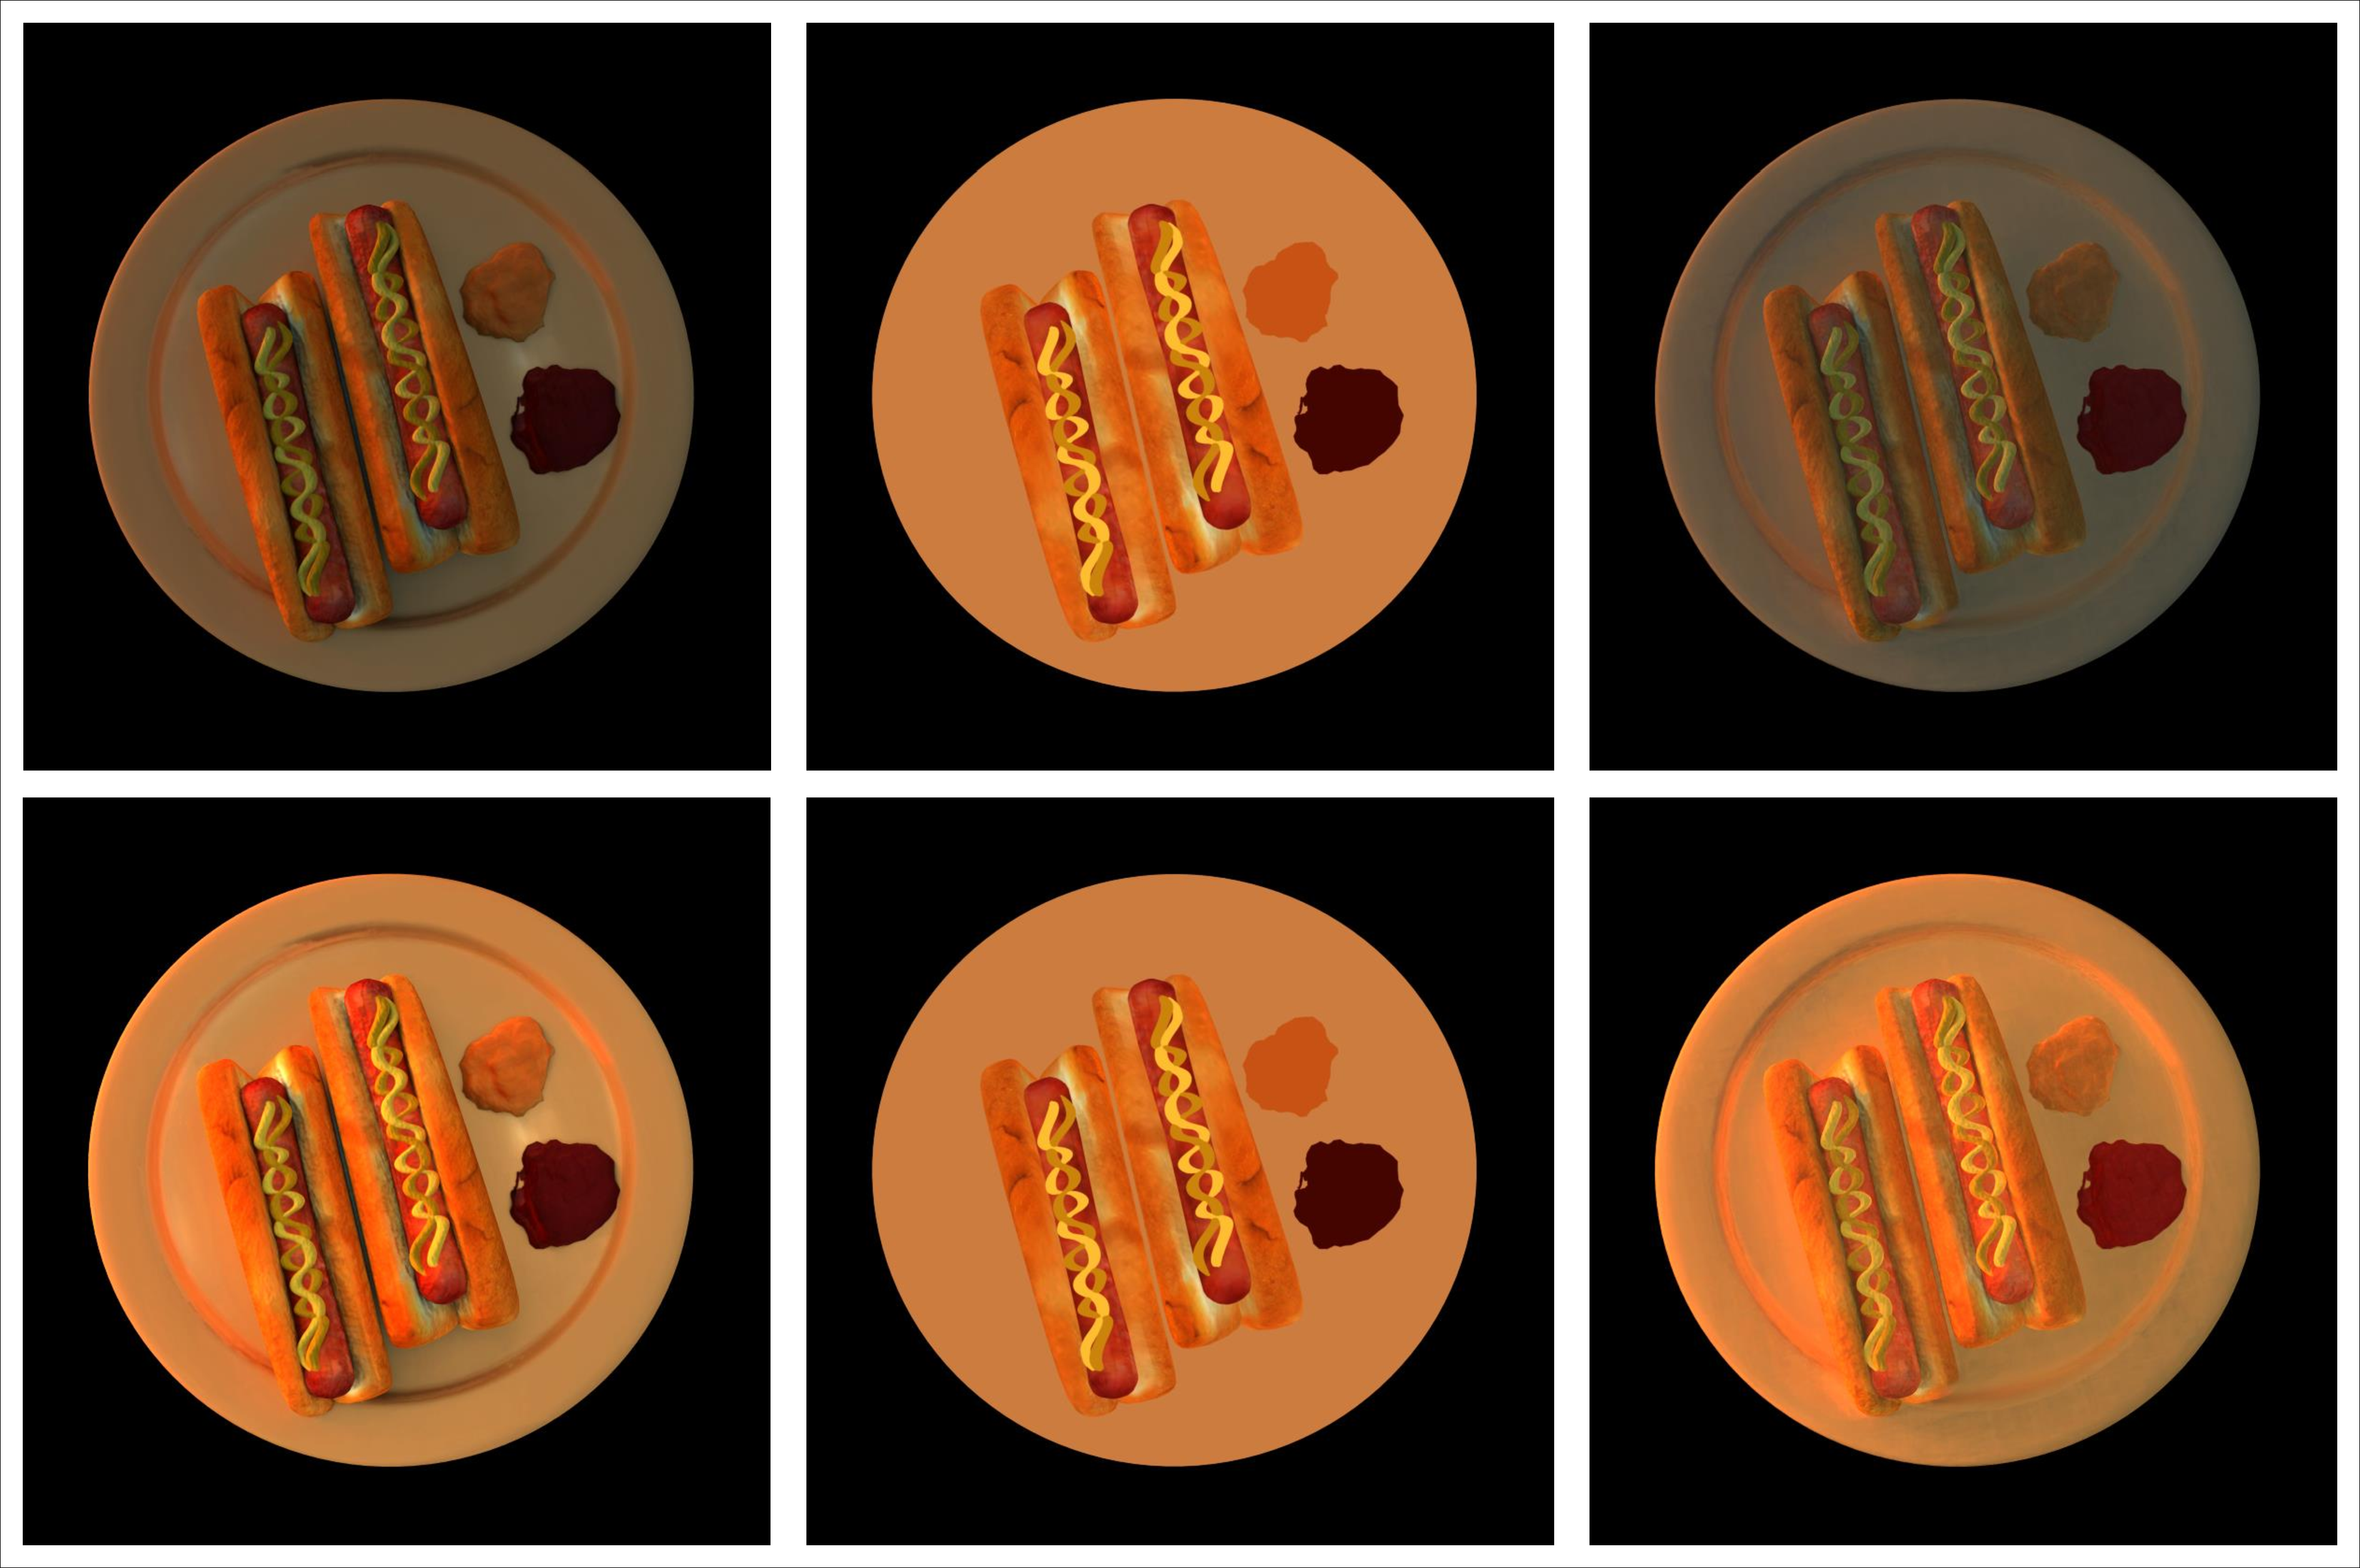
\includegraphics[width=\linewidth]{albedo.pdf}
  \caption{漫反射颜色比较}
  \label{fig:albedo}
\end{figure}

\begin{figure}[h]
  \centering
  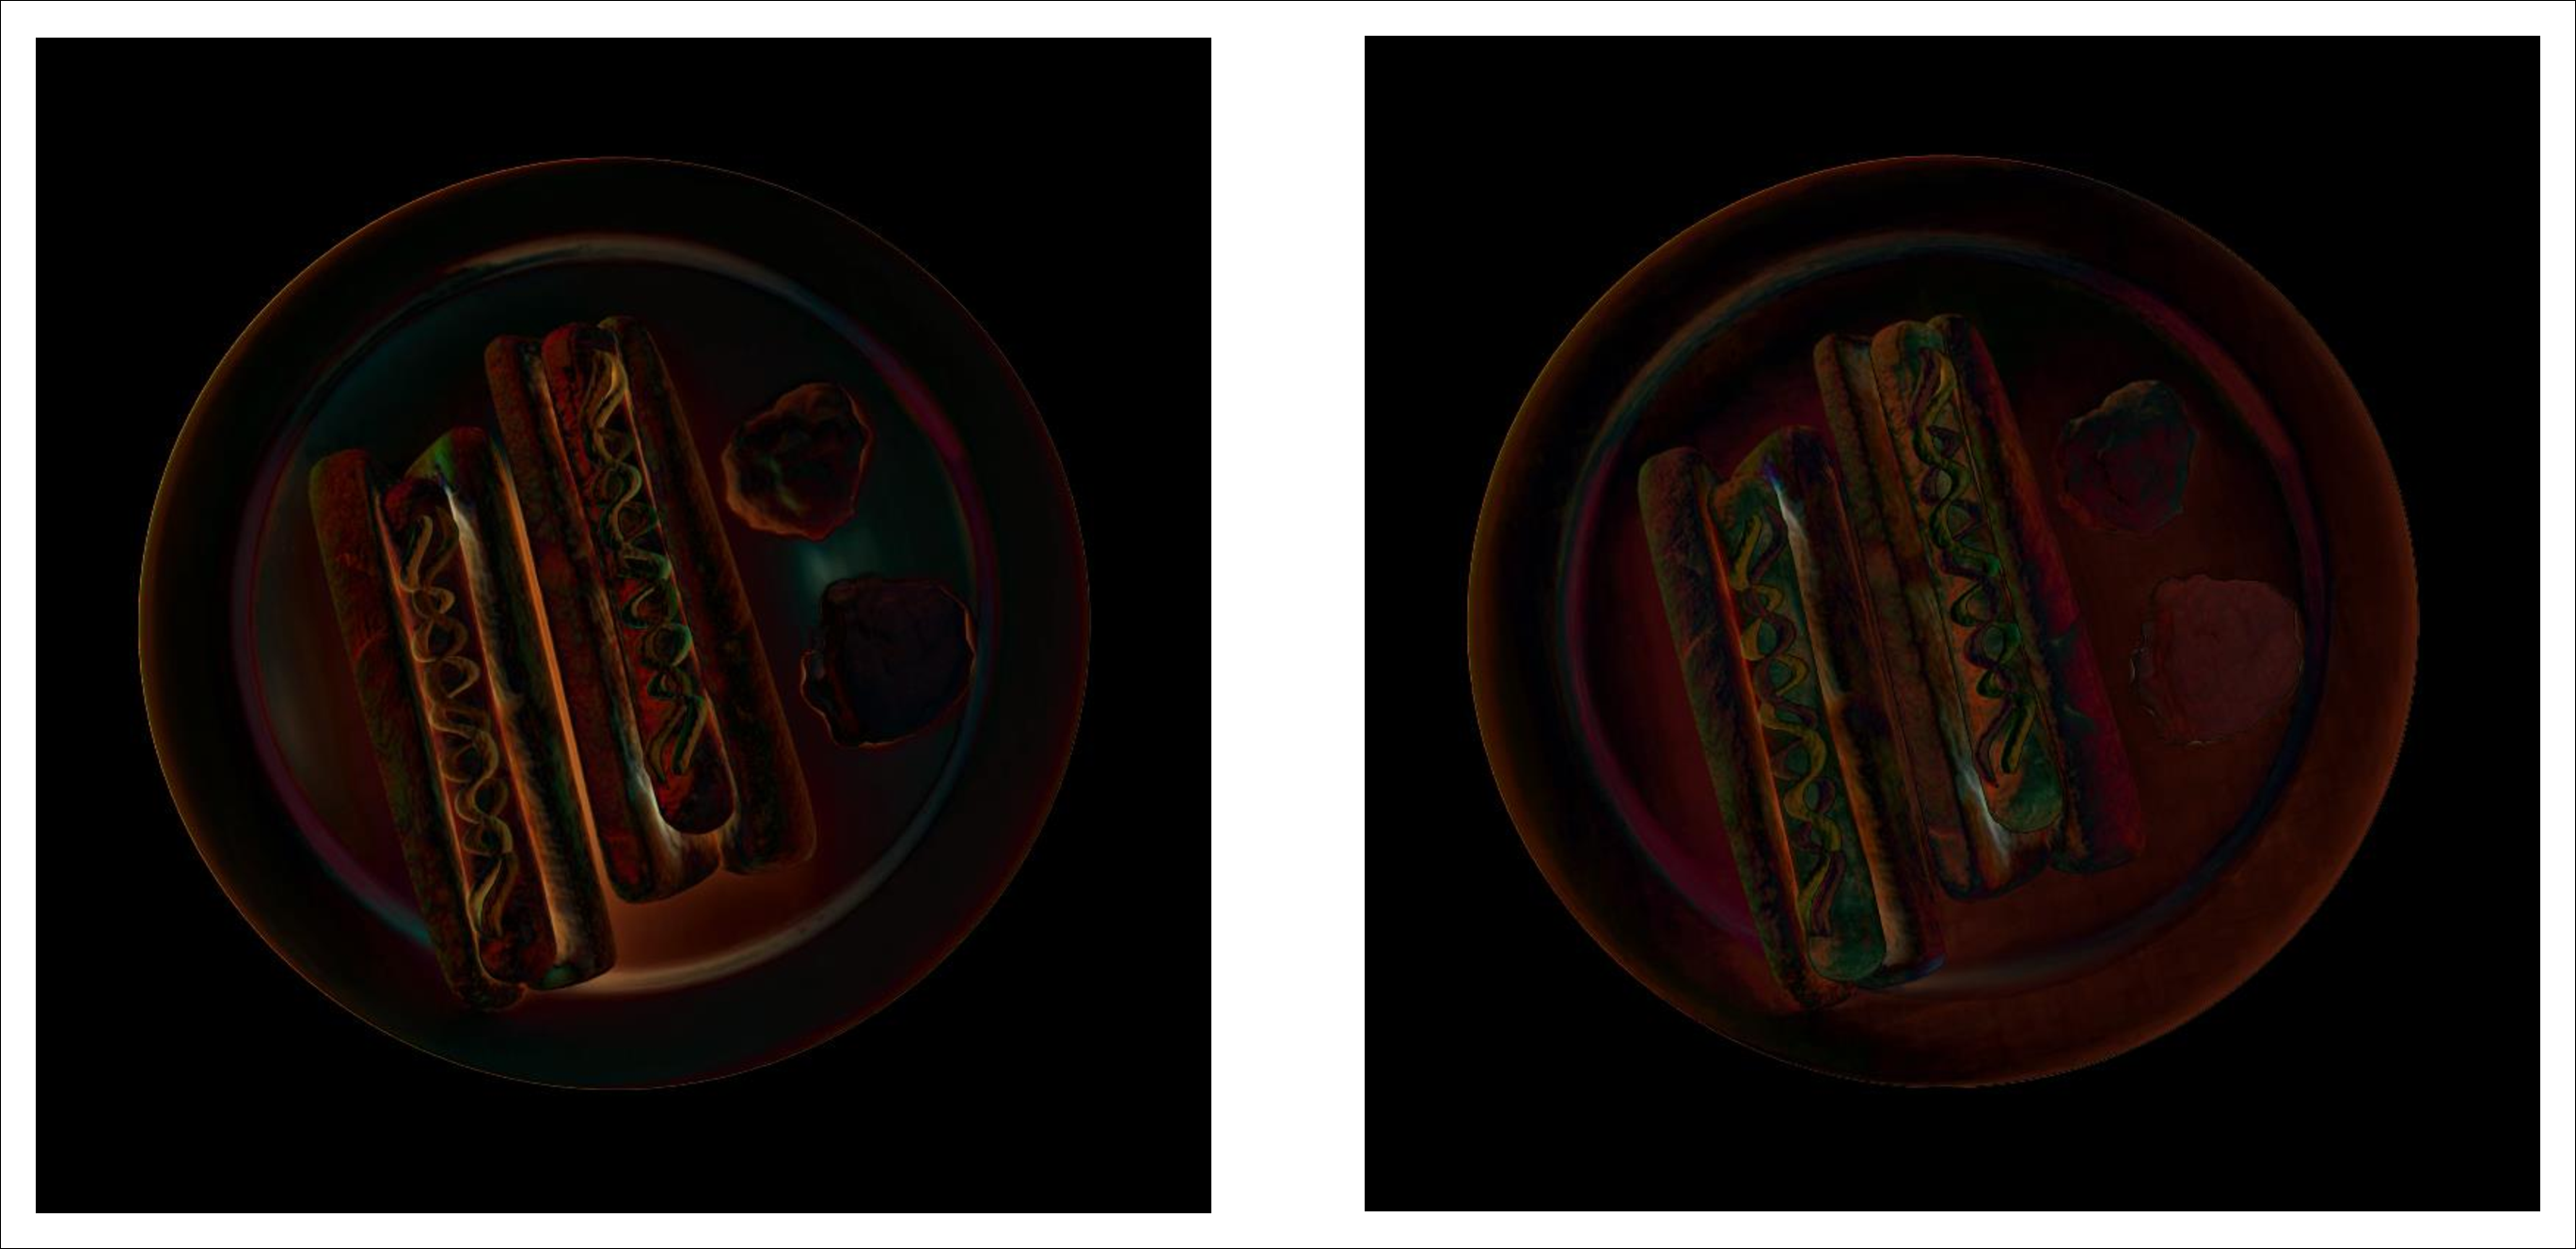
\includegraphics[width=0.81\linewidth]{diff.pdf}
  \caption{漫反射颜色比较2}
  \label{fig:diff}
\end{figure}

这一阶段训练的效果可以在图 \ref{fig:diff} 中更明显地看到。我们将加入第三阶段训练前后的漫反射颜色,在经过颜色修正后,直接与真实漫反射颜色作差得到图中的两张图片。可以看到,左图中有明显的亮区,对应着原图中照明伪影较多的区域。右图中则相对较少。
\chapter{总结与展望}

我们介绍了一种新颖的逆渲染方法,通过高质量的预处理和反复交替的可微光栅化和可微光线追踪,能够从多视角图像中重建高质量的水密流形三维网格,还原尽量真实的纹理贴图和环境光照,并主动从漫反射颜色中消除照明伪影。根据在仿真数据集上的实验,我们的方法在新视角合成和材质恢复方面表现出色。就我们所知,这项工作是目前第一个主动消除照明伪影的逆渲染方法。

我们的模型分为三个阶段。在第一阶段训练中,我们通过修改版 TensoIR,得到了三维密度场及神经网络表示的光照和材质网络。我们将其作为后续训练的高质量初始化。在第二阶段训练中,我们通过可微光栅化,将三维密度场转化为水密流形三维网格表示,并获得了与之对应的纹理和环境光照。在第三阶段训练中,我们通过可微光线追踪,优化了材质和环境光照,以消除照明伪影。我们的模型在这三个阶段的训练中,逐渐优化了三维密度场、材质和环境光照,最终得到了高质量的三维重建结果。

尽管取得部分成果,我们的方法尚有许多不足之处。首先,我们仍未在真实数据集上进行实验,因此我们的模型在真实场景中的表现尚不明确。其次,我们的模型由于引入可微光线追踪,训练速度较慢,仅仅第三阶段的训练每次大约需要二十小时。尽管在我们的任务中,这样的训练时间是可以接受的,但是在实际应用中效率也是一个重要的考量因素。再次,我们对去除照明伪影的效果仍不完全明确。我们需要设计更好的评价指标,来评估我们的模型在去除照明伪影方面的效果。如果能够按照材质对物体本身进行分割,甚至生成每个部件对应地几何结构和纹理贴图,将会使我们的模型更加完善。最后,我们的模型对物体材料和环境光照仍有较多限制。例如,我们的模型无法处理透明物体,也无法处理环境光照过强的情形。这也是由于逆渲染问题本身的不适定性。我们期望通过增加旋转光照等方式,为该问题添加更多的约束,以更好的实现还原真实材质、得到高质量三维模型的任务。



% 其他部分
% \backmatter

\listoffigures           % 插图清单
\listoftables            % 附表清单
% 参考文献
\bibliography{ref/refs}  % 参考文献使用 BibTeX 编译
% \printbibliography       % 参考文献使用 BibLaTeX 编译

% 致谢
% !TeX root = ../thuthesis-example.tex

\begin{acknowledgements}
  感谢杜韬教授和加州大学圣迭戈分校的苏昊教授在该项目上的指导和帮助,以及平时生活中对我的关心和支持。他们的悉心指导和耐心教诲使我受益匪浅。更重要的是,在与他们相处的过程中,我感受到了科研人对研究的热情、对生活的热爱和为人处世的态度。杜教授的温文尔雅和苏教授对于生活的热情都让我深深敬佩与向往。

  此外,我还要感谢弋力教授和段岳圻教授在我科研道路上的指导和帮助,以及关于职业规划和人生选择上的建议和支持。我还要感谢实验室的其他同学们,你们的帮助和支持使我在科研道路上走得更远。

  我还要感谢在清华四年中遇到的其他朋友们,以及计科03班级的其他同学们。与你们的交流让我成长为更充实丰满的自己,与你们的相处也让我的大学四年变得丰富多彩。我相信我们的友谊会一直延续下去。

  我要感谢同样热爱足球的朋友们。作为大学里最重要的爱好,足球让我们之间的羁绊变得更紧更深。我会永远记得每一场赢球后的欢呼雀跃,也会记得忙碌四年仍未升甲的遗憾和坐在紫操边上落寞的夜晚。

  我也要感谢紫二104B的兄弟们。我们一起度过了大学四年的难忘时光,也结下了深厚的友谊。除了在生活学习上的互帮互助,我也非常怀念玩耍、争论、欢笑与共同成长的日子。也许有些幽默的话语和深夜的辩论看起来有些许幼稚,但我相信这些都会成为我最宝贵的回忆。我衷心的认为我们宿舍是紫荆二号楼一层105B对面的宿舍中最好的宿舍,没有之一。

  我必须感谢我的女朋友。我很庆幸能在对的时间遇到最合适的你。在大学四年的时光里,我们一起制造浪漫,分享快乐,也一同面对生活学习的压力,一同经历困难与挫折后成长。你的支持和鼓励让我有勇气去承担更多的责任,有信心去铺设好我们的未来。在科研道路上的良师益友们让我成为了一个更好的学者,而你则让我成为了一个更好的人。

  我一定要感谢我的父母。你们将我从一个呱呱坠地的婴童抚育成人,给予我无微不至的爱和关怀,让我在正确的道路上长大成人。你们的教诲和以身作则塑造了我的血肉和人格,你们的支持和鼓励则让我可以无忧无虑地追求自己的梦想。我永远感激你们对我的付出和信任,也永远爱你们。

  最后,我要感谢每一个读到这里的读者,感谢你们的认可。我要感谢二十多年人生中的每一个面孔,即使我们只相逢一瞬。我要感谢清华大学,感谢这所美丽的大学中的一砖一瓦,一草一木。我要感谢每一个日出和日落,感谢每一个曾经的美好的梦。感谢生活。感谢世界。

\end{acknowledgements}


% 声明
% 本科生开题报告不需要
% \statement

% 附录
% 本科生需要将附录放到声明之后,个人简历之前
\appendix
% % !TeX root = ../thuthesis-example.tex

\begin{survey}
\label{cha:survey}

\title{Title of the Survey}
\maketitle

\tableofcontents

\section{Neural field representations.} Neural field representations mark an innovative departure from conventional methods such as meshes, volumes, and point clouds, heralding a paradigm shift in 3D content generation and modeling. The adaptability and precision of field representation render it remarkably proficient in replicating real-world scene geometry and appearance. Particularly noteworthy are seminal approaches like NeRF \cite{nerf} and subsequent developments such as Mip-NeRF \cite{mipnerf} and Tensor-NeRF \cite{tensorf}, which have introduced high-fidelity rendering capabilities, especially in novel view synthesis and diverse applications.

While many neural field representations portray 3D geometry as a density field primarily for rendering purposes, recent advancements advocate volumetric Signed Distance Fields (SDFs) as a superior alternative for enhanced surface reconstruction in volume rendering. However, challenges persist in exporting both density- and SDF-based models as meshes, resulting in a discernible degradation of rendering quality. Our work comprehensively tackles this challenge by introducing a solution that transforms volumetric neural field representations into high-quality manifold meshes. This transformation not only ensures exceptional rendering quality but also expands the scope of 3D applications, including physical simulation. Moreover, the capability to export meshes alongside corresponding materials, textures, and lighting conditions contributes to expedited rendering speeds.

\section{Differentiable ray tracing.} Ray tracing stands as a classical, pivotal, and highly effective rendering technique capable of accurately modeling illumination and yielding 100\% precise rendering outcomes. However, the realm of differentiable ray tracing presents a considerable challenge due to the presence of Dirac delta terms in the derivative of the integrand at occlusion boundaries, posing a significant hurdle for traditional sampling methods.

Prior research efforts \cite{N3MR, OpenDR} have addressed this challenge by resorting to simpler rendering models that overlook secondary effects such as shadows and indirect illumination. Another innovative approach proposed in \cite{DiffMCRT} involves explicit sampling of triangle edges, necessitating novel spatial acceleration strategies and importance sampling techniques. Furthermore, \cite{Mitsuba3} introduces a differentiable ray tracing system leveraging its own Dr.Jit compiler to expedite both the ray tracing process and its inverse counterpart. While some works resort to finite differences, which may suffice for straightforward geometries, they fail to offer a comprehensive solution to the complete light transport equation. Given the complexities involved in calculating derivatives with respect to geometry and optimizing meshes, we opt to maintain fixed geometry while optimizing other parameters such as lighting and materials to achieve better outcomes.

\section{Differentiable rasterization.} Differentiable rasterization stands as a pivotal paradigm in the fields of computer graphics and computer vision, offering a fresh approach to bridging the gap between traditional rendering methods and modern deep learning techniques. This method encompasses various strategies that imbue rasterization processes with differentiability, facilitating seamless integration into end-to-end differentiable pipelines.

In differentiable rasterization, geometric attributes such as vertices, edges, and faces are treated as continuous variables, enabling the computation of gradients with respect to these attributes. This enables neural networks to seamlessly incorporate rasterization, allowing the network to directly learn and optimize geometric attributes from image data.

In this study, we focus on investigating nvdiffrast \cite{nvdiffrast}, a comprehensive framework comprising four distinct stages: rasterization, interpolation, texture lookup, and anti-aliasing. Our primary emphasis lies in the rasterization stage, responsible for transforming geometric triangles from the three-dimensional domain to their corresponding positions in pixel space. Additionally, we pay particular attention to the interpolation stage, which provides the necessary three-dimensional pixel coordinates required for querying the appearance network.

\section{Inverse rendering.} Numerous studies \cite{d3c, xdd, svb} have proposed methods for inferring the geometry and material properties of real-world objects using collections of images. However, these approaches often require controlled lighting conditions or rely on learned domain-specific priors to address ambiguities in inverse rendering. In contrast, our work aims to estimate geometry, materials, and lighting simultaneously from images captured under unknown lighting conditions.

While neural representations have been applied to inverse rendering tasks, they face limitations due to the computation-intensive MLP architecture. This constraint poses a significant computational burden, especially when calculating secondary shading effects like shadows, which necessitate extensive sampling of secondary rays. To overcome this challenge, we employ an advanced TensoRF \cite{tensorf} representation that utilizes factorized tensors, enabling rapid reconstruction. Our TensoRF-based approach facilitates swift density and radiance evaluation, allowing for efficient real-time computation of secondary effects. Consequently, we achieve more accurate modeling of shadows and indirect lighting during the reconstruction process, thereby enhancing overall reconstruction accuracy.

% 默认使用正文的参考文献样式;
% 如果使用 BibTeX,可以切换为其他兼容 natbib 的 BibTeX 样式。
\bibliographystyle{unsrtnat}
% \bibliographystyle{IEEEtranN}

% 默认使用正文的参考文献 .bib 数据库;
% 如果使用 BibTeX,可以改为指定数据库,如 \bibliography{ref/refs}。
\printbibliography

\end{survey}
       % 本科生:外文资料的调研阅读报告
% \input{data/appendix-translation}  % 本科生:外文资料的书面翻译
% !TeX root = ../thuthesis-example.tex

\chapter{补充内容}

\section{现有可微光线追踪算法比较分析} \label{sec:compare}

在选择自行实现可微光线追踪框架前,我们调研并比较了多个现有可微光线追踪算法框架,主要包括 Mitsuba3 \cite{Mitsuba3}、Pyredner \cite{DiffMCRT}、Psdr-jit \cite{psdrjit}。下面我们对其进行简要的比较分析。

\subsection{Mitsuba3}

Mitsuba3 是由 Wenzel Jakob 等人开发的一款基于物理的渲染器,支持多种渲染算法,包括光线追踪、路径追踪、双向路径追踪等。该渲染器的计算框架基于Dr.Jit \cite{Drjit},这是一个高效的、用于数值计算和自动微分的库,使Mitsuba3能够实现可微光线追踪。这种能力使得它在计算机图形学和计算机视觉领域,特别是在需要梯度信息的优化任务中,具有极高的应用价值。

Mitsuba3 的一个显著优点是其Python接口封装得非常好,使得用户可以方便地调用各种功能。然而,尽管Mitsuba3在多方面表现出色,但其与PyTorch的兼容性却存在一定的问题。由于 Mitsuba3 基于 Dr.Jit,其与 Pytorch 并不兼容,梯度之间的传递非常困难。虽然 Mitsuba3 提供了一些可以与Pytorch兼容的方法,但是仍旧无法完全解决兼容问题。此外,非常好的封装性也意味着我们很难实现自定义模块。

我们的主要模型都是基于 Pytorch 框架实现的。我们尝试通过导出纹理图并单独使用 Mitsuba 优化,以将两者分开,然而这种方法并不高效,并且在导出纹理图时会产生误差,导致结果并不令人满意。

\subsection{Pyredner}

Redner 是由 Tzu-mao Li 等人开发的可微渲染器,Pyredner 是它的 python 版本。这个渲染器主要依照论文 Differentiable Monte Carlo Ray Tracing through Edge Sampling \cite{DiffMCRT} 实现。

Pyredner 本身依赖 Pytorch 框架进行开发,因此很容易与我们的模型兼容。Pyredner 的优点在于其简单易用,而且支持多种渲染算法,包括光线追踪、路径追踪等。然而,Pyredner 也存在一些问题,例如其文档不够完善,很多功能没有详细的说明,使得用户很难使用。关键问题在于,Pyredner 在2020年已经停止更新,这也导致其与最新版本的硬件不适配。我们也很难在 Pyredner 的基础上进行二次开发来满足我们的需求。

\subsection{Psdr-jit}

Psdr-jit是一款强大的可微渲染框架,顾名思义,这个框架同样基于Dr.Jit计算框架构建而成。它的前身是 Psdr-cuda,是一款基于物理的可微渲染器,用 C++17/CUDA 编写,并基于论文 Path-Space Differentiable Rendering \cite{PSDR} 实现。相较于其他两个渲染器,Psdr-jit 相对轻量级,同时他也支持GPU加速以及关于任意场景参数的梯度计算。

然而,与 Mitsuba3 类似,Psdr-jit同样基于 Dr.Jit 计算框架,导致梯度传递出现困难。此外,由于这是一个两人开发的小型渲染器,其说明文档并不完善,使得用户很难使用。因此我们无法选择 Psdr-jit 作为我们的基础框架。

\printbibliography


% 将签字扫描后的声明文件 scan-statement.pdf 替换原始页面
% \statement[file=scan-statement.pdf]
% 本科生编译生成的声明页默认不加页脚,插入扫描版时再补上;
% 研究生编译生成时有页眉页脚,插入扫描版时不再重复。
% 也可以手动控制是否加页眉页脚
% \statement[page-style=empty]
% \statement[file=scan-statement.pdf, page-style=plain]

% 个人简历、在学期间完成的相关学术成果
% 本科生可以附个人简历,也可以不附个人简历
% \input{data/resume}

% 指导教师/指导小组评语
% 本科生不需要
% \input{data/comments}

% 答辩委员会决议书
% 本科生不需要
% \input{data/resolution}

% 本科生的综合论文训练记录表(扫描版)
% \record{file=scan-record.pdf}

\end{document}
